% Usage: knitr slide

\chapter{Statistical Inference}\abd{6}\bmovie{4}\ddisc{4}
\section{Overview}
\bi
\item Inferential modes
  \bi
  \item hypothesis testing
  \item relative model fit/relative support for hypotheses (likelihood
    ratios, Bayes factors) 
  \item estimation (including interval estimation; often more appropriate than hypothesis testing) 
  \item Bayesian probability of an effect in the right direction (more
    relevant to decision making; more actionable)
  \ei
\item Contrast inference with decision making:
  \bi
  \item acting \emph{as if something is true} whether or not it is
    actually true
  \ei
\item Hypothesis testing is most useful for inferential ``existence'' questions
  \bi
  \item is indirect for other types of questions
  \ei
\item Majority of hypothesis tests are on a single point
\item These place asymmetric importance on ``special values'' such as
    zero treatment effect
\item What does it mean to ``not reject a hypothesis''?
  \bi
  \item often very little
  \ei
\item What does it mean to reject a hypothesis with a statistical test?
  \bi
  \item in statistics it means that \emph{some} aspect of a model is
    under suspicion (e.g., normality assumption)
  \item even if all other assumptions of the data model are satisfied,
    when the hypothesis involves a single point (e.g. zero 
    effect), the alternative space is infinite so what have we learned
    about a \emph{specific} alternative (e.g., that a treatment lowers
    blood pressure by 10 mmHg)?
  \ei
\ei

Statistical hypothesis testing involves a model for data:
\bi
\item Parametric tests have very specific models
\item Nonparametric tests have semi-specific models without a distribution assumption 
\item Permutation tests make an assumption about the best
  data summarization (e.g., mean, and the mean may not be the best
  summary for a heavy-tailed data distribution)
\ei

This chapter covers parametric tests for the following reasons:
\be
\item historical
\item they are very useful for sample size estimation
\item occasionally one has prior information that the raw data, or
  differences from pre to post, actually follow a normal distribution,
  and with large effects one can get quite significant results in very
  small samples with parametric tests
\item to show that Bayesian parametric tests make fewer assumptions
  about the data model
\ee
Nonparametric methods are covered in Chapter~\ref{chap:nonpar}. 

Back to data model---the primary basis for statistical inference:
\bi
\item Assume a model for how the data were generated
\item Model contains
  \bi
  \item main parameters of interest (e.g., means)
  \item auxiliary parameters for other variables (e.g., confounders)
  \item parameters for sources of between-subject variability
  \item if parametric, a distribution function such as Gaussian (normal)
  \item if nonparametric/semiparametric, a connection between
    distributions for different types of subjects (link function)
  \item if longitudinal, a correlation pattern for multiple
    measurements within a subject
  \item assumptions about censoring, truncation, detection limits if applicable
  \item \ldots
  \ei
\item Example (2-sample $t$-test): $Y = \mu_{0} + \delta
  [\textrm{treatment B}] + \epsilon$
  \bi
  \item $\mu_{0}$: unknown data-generating mean for treatment A
  \item $\delta$: unknown data-generating difference in means (B-A)
  \item $[\textrm{treatment B}]$: an indicator variable (1 if
    observation is from treatment B, 0 if from treatment A)
  \item $\epsilon$: irreducible error, i.e., unaccountable
    subject-to-subject variation; biologic variability; has variance $\sigma^2$
  \item \textbf{Primary goal}: uncover the hidden value of $\delta$
    generating our dataset in the presence of noise $\epsilon$
    \bi
    \item higher $\sigma^{2} \rightarrow$ larger $|\epsilon| \rightarrow$ harder
      to uncover $\delta$ (the signal) from the noise
    \item were $\epsilon$ always zero (no uncertainties), one
      \emph{directly observes} $\delta$ and no statistical analysis is needed
    \ei
  \ei
\item Rejecting a straw-man hypothesis implies that \emph{some} aspect of the
  model is in doubt
  \bi
  \item that aspect may be the distribution or an assumption about
    equal variances, not the difference in means you care about
  \ei
\ei

\textbf{Common error}: Using a two-stage approach to select which data
model to use:
\bi
\item Assumes the data contain rich enough information to lead to a
  correct decision
\item Alters the operating characteristics of the final test
\item Fails to realize that nonparametric tests have excellent power
\ei

Example: Testing normality to decide on whether to use a $t$-test
vs.\ a Wilcoxon-Mann-Whitney two-sample rank test.  A two-stage test
with a test for normality in the first stage assumes that
\be
\item the test for normality has power near 1.0 for our sample size
\item if the test rejects $H_{0}$:normality, the magnitude of
  non-normality is worth bothering about
\item pre-testing for normality does not modify the type I error of
  the overall testing procedure
\item nonparametric tests are less efficient than parametric tests
\ee
In fact it may be that none of these assumptions is true (4. is 
very seldom true).  As will be 
seen later, a full Bayesian model can be completely honest and provide
exactly the right amount of caution:
\bi
\item flexible parametric model allowing uncertainty about equal
  variances for groups A and B
\item allows uncertainty about the normality assumption
\item still results in inference about $\delta$, properly more
  cautious (wider credible interval) because
  \bi
  \item we don't know if normality truly holds
  \item we don't know if equality of variance truly holds
  \ei
\ei

\subsection{Central Limit Theorem}
\bi
\item Assume observations are independent with the same distribution
  and have finite variance
\item Assume that the sample size $n$ can increase without bound
\item Limiting distribution of the sample mean is normal
\ei

The CLT is frequently used to justify the use of parametric
statistical tests and confidence intervals even when their assumptions
are violated.  \textbf{But} the CLT (and the $t$ distribution) are
much less helpful for computing confidence intervals and $P$--values
than it seems~\cite{wil13avo}: 
\bi
\item since the standard deviation is unknown, one must estimate it
  while estimating the mean to use the CLT
\item SD may be a completely inappropriate summary of dispersion
  (e.g., if one should have first log-transformed but computed SD on
  the raw scale)
\item if the data distribution is asymmetric, the SD is not
  independent of the mean (so the $t$ distribution does not hold) and
  the SD is not a good dispersion measure
\item the sample size for which the CLT is an adequate approximation
  is unknown for any given situation
\item example: log-normal distribution---the CLT is not accurate even
  for $n=50000$ (see below) 
\item even when the CLT provides somewhat accurate $P$-values, it
  provides no comfort with regard to statistical power.  Example:
  analyzing $Y$ when you should have analyzed $\log(Y)$ will result in
  a devastating increase in type II error.
\ei

Example simulation to compute confidence-coverage when using the
$t$-distribution confidence interval for $n=50,000$ when analyzing
data from a log-normal distribution but not taking logs.  We want the
confidence limits to be such that the fraction of samples for which
the true population mean is to the left of the lower limit is 0.025,
and the fraction to the right of the upper limit to also be 0.025.

\begin{Schunk}
\begin{Sinput}
n    <- 50000
nsim <- 5000            # number of simulations
mul <- 0; sdl <- 1.65   # on log scale
mu <- exp(mul + sdl * sdl / 2)   # population mean on orig. scale
count <- c(lower=0, upper=0)
set.seed(1)
z <- qt(0.975, n - 1)   # t critical value (near 1.96)

for(i in 1 : nsim) {
  x <- exp(rnorm(n, mul, sdl))
  ci <- mean(x) + c(-1, 1) * z * sqrt(var(x) / n)
  count[1] <- count[1] + (ci[1] > mu)
  count[2] <- count[2] + (ci[2] < mu)
}

count / nsim   # non-coverage prob. in left and right tail
\end{Sinput}
\begin{Soutput}
 lower  upper 
0.0182 0.0406 
\end{Soutput}
\end{Schunk}

See
\href{https://stats.stackexchange.com/questions/204585}{stats.stackexchange.com/questions/204585}
for more information and discussion.

\section{Hypotheses}
\subsection{Scientific Hypotheses and Questions}
Scientific questions are usually stated with a direction or with
regard to an expected effect, not with respect to a null effect.
Scientific questions often involve estimating a quantify of interest.
Here are some examples:
\bi
\item Does the risk of death increase when serum triglyceride
  increases?
\item To what extent is mechanism $x$ responsible for regulation of physiologic
  parameter $y$?
\item What is the average decrease in blood pressure when the dose of
  a drug goes from 0 to 10mg/day to 20mg/day?
\ei
\subsection{Statistical Hypotheses}
\bi
\item Hypothesis: usually a statement to be judged of the form \\
  ``population value = specified constant''
 \bi
 \item $\mu = 120$mmHg
 \item $\mu_{1} - \mu_{2} = 0$mmHg
 \item Correlation between wealth and religiosity = 0
 \ei
\item Null hypothesis is usually a hypothesis of no effect but can be
 $H_{0}: \mu =$ constant or $H_{0}:$ Probability of heads
 $=\frac{1}{2}$; \\
 $H_{0}$ is often a straw man; something you hope to disprove
\item Alternative hypothesis: $H_1$; e.g.: $H_{1}: \mu \neq 120$mmHg
\item One-sided hypothesis (tested by 1-tailed test): $H_{1}$ is an
  inequality in one direction ($H_{1}: \mu > 120$mmHg)
\item Two-sided hypothesis (2-tailed test, most common type): $H_{1}$
  involves values away from the hypothesized value in either direction
\ei

\section{Branches of Statistics}\label{sec:htest-branches}
\bi
\item Classical (frequentist or sampling statistics)\ros{7.1-7.2}
 \bi
  \item Emphasizes (overemphasizes?) hypothesis testing
 \item Assumes $H_{0}$ is true and tries to amass evidence casting
   doubt on this assumption
 \item Conceives of data as one of many datasets that \emph{might} have
   happened; considers the process by which the sample arose
 \item Inference is based on long-run operating characteristics not
   about direct evidence from the sample at hand
   \bi
   \item probability of making an assertion of an effect if there is
     no effect
   \item proportion of the time that varying confidence intervals over replicates
     of the experiment cover the true unknown parameter; no statement
     about the chance that the 
     current confidence interval covers the true parameter
   \ei
 \item See if data are consistent with $H_{0}$
 \item Are data extreme or unlikely if $H_{0}$ is really true?
 \item Proof by contradiction: if assuming $H_{0}$ is true leads to
   results that are ``bizarre'' or unlikely to have been observed,
   casts doubt on premise
 \item Evidence summarized through a single statistic capturing a
   tendency of data, e.g., $\bar{x}$
 \item Look at probability of getting a statistic as or more extreme
   than the calculated one (results as or more impressive than ours)
   if $H_{0}$ is true (the $P$-value)\footnote{We could drop the
     ``as'' and just say ``more extreme'' because for continuous data
     the probability of getting a result exactly as extreme as ours is
     exactly zero.}
 \item If the statistic has a low probability of being more extreme we say
   that if $H_{0}$ is true we have acquired data that are very
   improbable, i.e., have witnessed a low probability event
 \item William Briggs in
   \href{https://wmbriggs.com/public/Briggs.EverthingWrongWithPvalues.pdf}{wmbriggs.com/public/Briggs.EverthingWrongWithPvalues.pdf}
   described a basic flaw in the logic of $P$-value-guided hypothesis
   testing dating all the way back to Fisher:\\
   {\smaller
A version of an argument given first by Fisher appears in every
introductory statistics book. The original argument is this,
[33]:\\~\\``Belief in a null hypothesis as an accurate representation of
the population sampled is confronted by a logical disjunction: Either
the null hypothesis is false, or the p-value has attained by chance an
exceptionally low value.''\\~\\
A logical disjunction would be a proposition of the type ``Either it
is raining or it is not raining.'' Both parts of the proposition
relate to the state of rain. The proposition ``Either it is raining or
the soup is cold'' is a disjunction, but not a logical one because the
first part relates to rain and the second to soup. Fisher's ``logical
disjunction'' is evidently not a logical disjunction because the first
part relates to the state of the null hypothesis and the second to the
p-value.  Fisher's argument can be made into a logical disjunction,
however, by a simple fix. Restated: Either the null hypothesis is
false and we see a small p-value, or the null hypothesis is true and
we see a small p-value. Stated another way, ``Either the null
hypothesis is true or it is false, and we see a small p-value.'' The
first clause of this proposition, ``Either the null hypothesis is true
or it is false'', is a tautology, a necessary truth, which transforms
the proposition to (loosely) ``TRUE and we see a small p-value.''
Adding a logical tautology to a proposition does not change its truth
value; it is like multiplying a simple algebraic equation by 1.  So,
in the end, Fisher's dictum boils down to: ``We see a small p-value.''
In other words, in Fisher's argument a small p-value has no bearing on
any hypothesis (any hypothesis unrelated to the p-value itself, of
course). Making a decision about a parameter or data because the
p-value takes any particular value is thus always fallacious: it is not
justified by Fisher's argument, which is a non sequitur.       
     } \\~\\
   Ignoring all that and plunging ahead:
 \item $P$-value is a measure of \emph{surprise} that is well described
   by Nicholas Maxwell\footnote{Data Matters: Conceptual Statistics
     for a Random World.  Emeryville CA: Key College Publishing, 2004.}:
   ``A p value is a measure of how embarrassing the data are to the null
   hypothesis''
 \item Then evidence mounts against $H_{0}$ and we might reject it
 \item A failure to reject \emph{does not} imply that we have gathered
   evidence in favor of $H_0$ --- many reasons for studies to not
   be impressive, including small sample size ($n$)
 \item Ignores \emph{clinical} significance
 \item Is fraught with how to deal with multiplicity problems
   \bi
   \item No principled recipe for how they should be handled
   \item Arise because
     \bi
     \item type I error is fixed at a number $> 0$
     \item backward time ordering of information (transposed conditional)
     \ei
   \item Evidence about one question is changed according to whether
     other questions are asked (regardless of their answers)
   \ei
 \ei
\item Classical parametric statistics: assumes the data to arise from
  a certain distribution, often the normal (Gaussian distribution)
\item Nonparametric statistics: does not assume a data distribution;
  generally looks at ranks rather than raw values
\item Bayesian statistics: \ros{7.8}
 \bi
 \item Considers the sample data, not how it arose from a sequence of
   samples but rather the data generating mechanism for \emph{this} sample
 \item Computes the probability that a clinically interesting
   statement is true, e.g. that the new drug lowers population mean
   SBP by at least 5mmHg, given what we observed in the data
 \item Instead of trying to amass evidence against a single
   hypothesized effect size, Bayes tries to uncover the hidden
   parameter generating the data aside from noise (e.g., treatment
   effect) whatever its value
   \bi
    \item Provides evidence for \emph{all possible values} of an unknown parameter
   \ei

 \item More natural and direct approach but requires more work
 \item Because respects forward flow of time/information there is no
   need for nor availability of methods for correcting for
   multiplicity\footnote{Bayesian inference assumes only that the
     prior distribution is ``well calibrated'' in the sense that one
     sticks to the pre-specified prior no matter what information is unveiled.}
 \item Evidence about one question is not tilted by whether other
   questions are asked
 \item Can formally incorporate knowledge from other studies as well
   as skepticism from a tough audience you are trying to convince to
   use a therapy
 \item Starting to catch on (only been available for about 240 years)
   and more software becoming available
 \ei
\item Likelihood inference\footnote{A key thinker and researcher in the field is Richard Royall.}:
  \bi
  \item Considers the sample data, not how it arose
  \item Akin to Bayesian but without the prior
  \item Interval estimates are based on relative likelihood (from the
    likelihood function) and are called likelihood support intervals
  \item For testing, allows both type I and type II errors
    $\rightarrow 0$ as $n \rightarrow \infty$, whereas with
    frequentist methods the type I error never shrinks as $n
    \rightarrow \infty$
  \item This greatly reduces problems with multiplicities
  \item Likelihood methods do not deal well with complex assertions
    (e.g., either the treatment reduces mortality by any amount or
    reduces blood pressure by at least 10 mmHg) and do not allow the
    use of external information
  \ei
\item Bayesian and likelihood inference use the \emph{likelihood
    principle}; frequentist inference does not 
 \bi
 \item Likelihood principle: All of the evidence in a sample relevant
   to model parameters is in the likelihood function 
 \item If we want to know our current location, frequentist inference
   asks the following: If I am in Nashville, what fraction of routes
   to here involved the southern route I took? 
   There are many paths to get where we are, and frequentists have to
   consider all possible relevant paths.  Bayesian and likelihood
   inference states it differently: Where am I now?  This involves an
   assessment of current evidence about my location.  Asking ``how did
   I get here?'' (i.e., how did the data arise?) involves multiplicity
   issues that answering the simpler question does not. 
\item Consider a sequentially monitored randomized experiment.
  Bayesians and likelihoodists can make infinitely many assessments of
  efficacy with no penalty.  On the other hand, a frequentist must
  think the following way:
  \begin{quote}
    I am at the first interim analysis.  I am going to make later
    assessments of efficacy so I need to discount the current
    assessment and be more conservative or I will spend all my
    $\alpha$ already.\\
    \ldots\\
    I am at the fifth interim analysis.  I made four previous efficacy
    assessments, and even though none of them mattered, I spent
    $\alpha$ so I need to discount the current assessment and be more
    conservative.
 \end{quote}
 \ei
\item We will deal with classical parametric and nonparametric
  statistical tests more than Bayesian methods just because of time
  and because of abundance of software for the former
\ei

\section{Errors in Hypothesis Testing; $P$ Values} \ros{7.2}\katz{7.5.A-7.5.B}
\bi
\item Can attempt to reject a formal hypothesis or just compute
  $P$-value
\item Type I error: rejecting $H_0$ when it is true \\
  $\alpha$ is the probability of making this error (typically set at
  $\alpha=0.05$---for weak reasons)
  \bi
  \item To be specific: $\alpha$ = P(asserting an
    effect exists when in fact it doesn't)
  \item So it is an assertion probability or false alarm probability
    like 1 minus specificity
  \item It \textbf{is not} a false positive probability (P(effect=0)
    given an assertion that it is nonzero) since $\alpha$ is based on
    an \textbf{assumption} that effect=0
  \ei
\item Type II error: failing to reject $H_0$ when it is false \\
  probability of this is $\beta$
\begin{center}
\begin{tabular}{|l||c|c|} \hline
 & \multicolumn{2}{|c|}{True state of $H_0$} \\ \hline 
Decision & $H_0$ true & $H_0$ false \\ \hline \hline
Reject $H_0$ & Type I error ($\alpha$) & Correct \\  \hline
Do Not Reject $H_0$ & Correct & Type II error ($\beta$) \\  \hline
\end{tabular}
\end{center}

\item Power: $1 - \beta$: probability of (correctly) rejecting $H_0$
  when it is false
\ei

Within the frequentist framework of statistics there are two schools.
One, the Neyman-Pearson school, believes that the type I error should
be pre-set at $\alpha$ (say $\alpha=0.05$) so that binary decisions
can be made (reject/fail to reject).  The other school due to Fisher
believes that one should compute $P$-values and quote the result in
the report or publication.  This is the more popular approach, being less dichotomous.

\bi
  \item Simplest definition of $\alpha$: probability that a $P$-value
    will be less than it
\ei


A $P$-value is something that can be computed without speaking of
errors.  It is the probability of observing a statistic as or more
extreme than the observed one if $H_0$ is true, i.e., if the
population from which the sample was randomly chosen had the
characteristics posited in the null hypothesis.\footnote{Note that
  Rosner's Equation 7.4 in his section 7.3 is highly 
problematic.  Classifications of ``significant'' or ``highly
significant'' are arbitrary, and treating a $P$-value between 0.05 and
0.1 as indicating a ``trend towards significance'' is bogus.  If the
$P$-value is 0.08, for example, the 0.95 confidence interval for the
effect includes a ``trend'' in the opposite (harmful) direction.}  The
$P$-value to have the usual meaning assumes that the data model is correct.

\subsection{Problems With Type I Error}
\bi
\item It's not really an ``error''
  \bi
  \item Error = being wrong in asserting an effect
  \item Type I = P(asserting effect $| H_{0}$) = ``effect assertion probability''
  \ei
\item Frequentist designs attempt to preserve type I error
\item This is not the probability of making a mistake in concluding an
  effect is present
\item When $\alpha=0.05$ the probability of asserting an effect when
  there is none never decreases even as $n \rightarrow \infty$
  \\ (statistical vs.\ clinical significance problem)
\item $\alpha$ does not depend on any observed data.  It is a
  pre-study concept.
\item $\alpha$ increases because of chances you give data to be more
  extreme (multiplicity), not because of chances you give hypotheses
  to be false.  Bayesian and likelihood approaches do not look at
  sampling (sample space giving rise to data extremes).  See
  \href{http://fharrell.com/post/bayes-seq}{\url{fharrell.com/post/bayes-seq}} 
\item Probability of making a mistake in asserting an effect, given
  the data, is one minus the Bayesian posterior probability of efficacy
\ei

\subsection{Misinterpretation of $P$-values}
$P$-values have come under extreme criticism since 2000, partially
because they are often misinterpreted. Greenland~\etal~\cite{gre16sta}
is the best paper that summarizes the misinterpretations and explains
them.  Some quotes from this paper are below, with their explanations
for the first two.

\begin{quote}
  \begin{enumerate}
  \item \textbf{The $P$ value is the probability that the test
      hypothesis is true; for example, if a test of the null
      hypothesis gave $P$ = 0.01, the null hypothesis has only a 1\%
      chance of being true; if instead it gave $P$ = 0.40, the null
      hypothesis has a 40\% chance of being true.} No! The $P$ value
    assumes the test hypothesis is true---it is not a hypothesis
    probability and may be far from any reasonable probability for the
    test hypothesis. The $P$ value simply indicates the degree to
    which the data conform to the pattern predicted by the test
    hypothesis and all the other assumptions used in the test (the
    underlying statistical model). Thus $P$ = 0.01 would indicate that
    the data are not very close to what the statistical model
    (including the test hypothesis) predicted they should be, while
    $P$ = 0.40 would indicate that the data are much closer to the
    model prediction, allowing for chance variation. 
  \item \textbf{The $P$ value for the null hypothesis is the
      probability that chance alone produced the observed association;
      for example, if the $P$ value for the null hypothesis is 0.08,
      there is an 8\% probability that chance alone produced the
      association.}  No! This is a common variation of the first
    fallacy and it is just as false. To say that chance alone produced
    the observed association is logically equivalent to asserting that
    every assumption used to compute the $P$ value is correct, including
    the null hypothesis. Thus to claim that the null $P$ value is the
    probability that chance alone produced the observed association is
    completely backwards: The $P$ value is a probability computed
    assuming chance was operating alone. The absurdity of the common
    backwards interpretation might be appreciated by pondering how
    the $P$ value, which is a probability deduced from a set of
    assumptions (the statistical model), can possibly refer to the
    probability of those assumptions. Note: One often sees ``alone''
    dropped from this description (becoming ``the $P$ value for the null
    hypothesis is the probability that chance produced the observed
    association''), so that the statement is more ambiguous, but just
    as wrong.
  \item \textbf{A significant test results ($P\leq 0.05$) means that
      the test hypothesis is false or should be rejected.} No!
  \item \textbf{A nonsignificant test results ($P > 0.05$) means that
      the test hypothesis is true or should be accepted.} No!
  \item \textbf{A large $P$ value is evidence in favor of the test
      hypothesis.} No!
  \item \textbf{A null-hypothesis $P$ value greater than 0.05 means
      that no effect was observed, or that absence of an effect was
      shown or demonstrated.} No!
  \item \textbf{Statistical significance indicates a scientifically or
      substantively important relation has been detected.} No!
  \item \textbf{Lack of statistical significance indicates that the
      effect size is small.} No!
  \item \textbf{The $P$ value is the chance of our data occurring if
      the test hypothesis is true; for example, $P$ = 0.05 means that
      the observed association would occur only 5\% of the time under
      the test hypothesis.} No!
  \item \textbf{If you reject the test hypothesis because $P \leq
      0.05$, the change you are in error (the chance your
      ``significant finding'' is a false positive) is 5\%.} No!
  \item \textbf{$P = 0.05$ and $P \leq 0.05$ mean the same thing.} No!
  \item \textbf{$P$ values are properly reported as inequalities (e.g., report ``$P < 0.02$'' when $P = 0.015$ or report $P > 0.05$ when $P = 0.06$ or $P = 0.70$).} No!
  \item \textbf{Statistical significance is a property of the phenomenon being studied, and thus statistical tests detect significance.} No!
  \item \textbf{One should always use two-sided $P$ values.} No!
  \item \textbf{When the same hypothesis is tested in different studies and none or a minority of the tests are statistically significant (all $P > 0.05$), the overall evidence supports the hypothesis.} No!
  \item \textbf{When the same hypothesis is tested in two different populations and the resulting $P$ values are on opposite sides of 0.05, the results are conflicting.} No!
  \item \textbf{When the same hypothesis is tested in two different populations and the same $P$ values are obtained, the results are in agreement.} No!
  \item \textbf{If one observes a small $P$ value, there is a good chance that the next study will produce a $P$ value at least as small for the same hypothesis.} No!
  \item \textbf{The specific 95\% confidence interval presented by a study has a 95\% chance of containing the true effect size.} No!
  \item \textbf{An effect size outside the 95\% confidence interval has been refuted (or excluded) by the data.} No!
  \item \textbf{If two confidence intervals overlap, the difference between the two estimates or studies is not significant.} No!
  \item \textbf{An observed 95\% confidence interval predicts that 95\% of the estimates from future studies will fall inside the observed interval.} No!
  \item \textbf{If one 95\% confidence interval includes the null value and another excludes that value, the interval excluding the null is the more precise one.} No!
  \item \textbf{If you accept the null hypothesis because the null $P$ value exceeds 0.05 and the power of your test is 90\%, the chance you are in error (the chance that your finding is a false negative) is 10\%.} No!
  \item \textbf{If the null $P$ value exceeds 0.05 and the power of this test is 90\% at an alternative, the results support the null over the alternative.} \dots counterexamples are easy to construct \dots
 \end{enumerate}
\end{quote}

\section{Interval Estimation}
\subsection{Frequentist Confidence Intervals}
A $1-\alpha$ two-sided confidence interval is an interval computed such that
\bi
\item if the experiment were repeated $N$ times one would expect $N \times (1 - \alpha)$ of the recomputed varying intervals to contain the true unknown quantity of interest 
\item equivalently the set of all unknown population parameter values that if null hypothesized one would not reject that null hypothesis at the $\alpha$ level in a two-sided test
  \bi
  \item e.g. when estimating the population mean $\mu$, the set $\mu_{0}$ such that the test $H_{0}: \mu = \mu_{0}$ has a $P$-value $> \alpha$
  \ei
  For this reason confidence intervals may better be called \emph{compatibility intervals}.
\ei

\textbf{Pros}:
\bi
\item The $P$-value can be computed from the confidence interval but not vice-versa, so confidence limits have more information
\item Confidence intervals do not allow the ``absence of evidence is not evidence of absence error''
  \bi
  \item large $P$-values can come from small $n$ or large $\sigma^2$
  \item these make confidence intervals wide, giving a rational sense of uncertainty 
  \item A confidence interval that is compatible with both large benefit and large detriment indicates that we don't know much
    \bi
    \item large $P$-value means nothing more than ``get more data''
    \ei
\ei
\ei

\textbf{Cons}:
\bi
\item Confidence intervals have only a long-run interpretation over many experiments
\item They don't provide a probability statement about whether a single interval includes the true population value
  \bi
  \item In the frequentist world, the probability that the parameter is in a given interval is either zero or one
  \ei
\item They are often taken to provide a measure of precision of a statistical estimate, but they're not really that either
\item The experimenter controls the long-run inclusion probability $1 - \alpha$ and gets interval endpoints, but is often more interested in the probability that the population effect is in a pre-chosen fixed interval
\item It is very difficult to make confidence intervals incorporate known uncertainties (e.g., amount of non-normality), making them often too narrow (overoptimistic)
\ei  
 
\subsection{Bayesian Credible Intervals}
\bi
\item Credible intervals have the interpretation that most researchers seek when they compute confidence intervals
\item A $1 - \alpha$ credible interval is an interval $[a, b]$ (computed, under a certain prior distribution encapsulating prior knowledge about the parameter $\mu$) so that \\ $P(a \leq \mu \leq b | \textrm{ data}) = 1 - \alpha$
\ei

\textbf{Pros}:
\bi
\item Pertains to the single, current dataset and does not provide just long-run operating characteristics
\item Provides a true probability statement even when the experiment could never be repeated
\item Is symmetric with Bayesian posterior probabilities of pre-chosen limits
  \bi
  \item Researchers can specify $a, b$ and then compute whatever probability it is that the unknown parameter is in that interval
  \ei
\item The credible interval can take into account all sorts of uncertainties (e.g., non-normality) that make it (correctly) wider
\ei

\textbf{Cons}:
\bi
\item One must specify a prior distribution
\ei

\section{One Sample Test for Mean} \ros{7.3-7.4,7.12}\bmovie{5}\ddisc{5}
\subsection{Frequentist Method}
\bi
\item Assuming continuous response from a normal distribution
\item One sample tests for $\mu =$ constant are unusual except when
  data are paired, e.g., each patient has a pre-- and post--treatment
  measurement and we are only interested in the mean of post - pre
  values
\item $t$ tests in general:
\beq
t = \frac{\textrm{estimate - hypothesized value}}{\textrm{standard deviation
  of numerator}}
\eeq
\item The standard deviation of a summary statistic is called its
  \emph{standard error}, which is the $\sqrt{}$ of the variance of the
  estimate 
\item The one-sample $t$ statistic for testing a single population
  mean against a constant $\mu_0$ ($H_{0}$: $\mu = \mu_{0}$; often
  $\mu_{0} = 0$) is 
\beq
t = \frac{\bar{x} - \mu_{0}}{se}
\eeq
where $se = \frac{s}{\sqrt{n}}$, is the standard error of the mean (SEM) and $\bar{x}$ is the sample mean

%because the variance of $\bar{x}$ is the variance of an individual $x$ value divided by the number of values being averaged $\rightarrow \sigma^{2}/n$
% \bi
% \item If you repeated an experiment $M$ times, each time computing
%   $\bar{x}$ from $n$ observations, the $M \bar{x}$s would vary
%   $\frac{1}{n}$th as much as the raw measurements vary between
%   patients
% \ei
\item When your data comes from a normal distribution and $H_{0}$ holds, the
  $t$ ratio \textbf{statistic} follows the $t$ \textbf{distribution}
\item With small sample size ($n$), the $t$ ratio is unstable because the sample standard deviation ($s$) is not
  precise enough in estimating the population standard deviation ($\sigma$; we are assuming that $\sigma$
  is unknown)
\item This causes the $t$ distribution to have heavy tails for small
  $n$
\item As $n\uparrow$ the $t$ distribution becomes the normal
  distribution with mean zero and standard deviation one
\item The parameter that defines the particular $t$ distribution to
  use as a function of $n$ is called the \emph{degrees of freedom} or
  d.f.
\item d.f. = $n$ - number of means being estimated
\item For one-sample problem d.f. = $n-1$
\item Symbol for distribution $t_{n-1}$

\begin{Schunk}
\begin{Sinput}
x <- seq(-3, 3, length=200)   # Fig. (*\ref{fig:htest-tpdfs}*)
w <- list(Normal     = list(x=x, y=dnorm(x)),
          't (50 df)'= list(x=x, y=dt(x, 50)),
          't (5 df)' = list(x=x, y=dt(x, 5)),
          't (2 df)' = list(x=x, y=dt(x,2)))
labcurve(w, pl=TRUE, keys='lines', col=c(1,2,4,5), lty=c(2,1,1,1),
         xlab=expression(x), ylab='')
\end{Sinput}
\begin{figure}[htbp]

\centerline{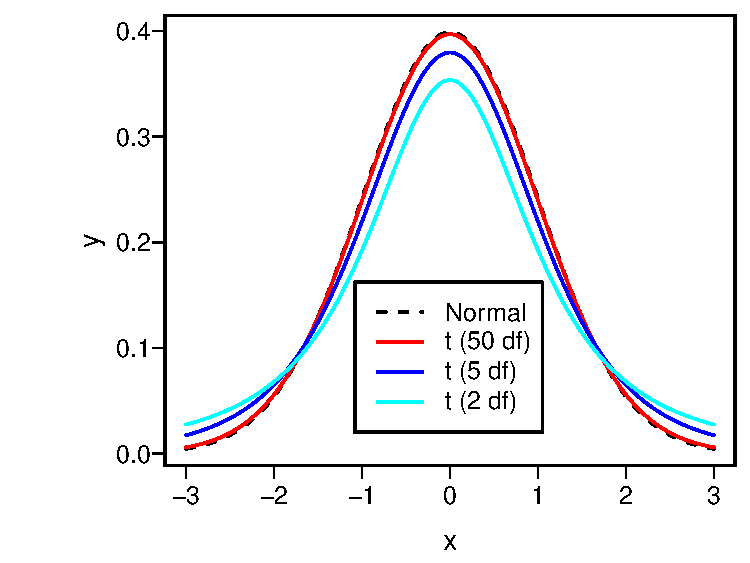
\includegraphics[width=\maxwidth]{htest-tpdfs-1} }

\caption[$t$ distribution for varying d.f.]{Comparison of probability densities for $t_2$, $t_5$, $t_{50}$, and normal distributions}\label{fig:htest-tpdfs}
\end{figure}
\end{Schunk}

\item Two-tailed $P$-value: probability of getting a value from the
  $t_{n-1}$ distribution as big or bigger in absolute value than the
  absolute value of the observed $t$ ratio
\item Computer programs can compute the $P$-value given $t$ and
  $n$.\footnote{\R\ has the function \texttt{pt} for the cumulative
    distribution function for the $t$ distribution, so the 2-tailed
    $P$-value would be obtained using 
    \texttt{2*(1-pt(abs(t),n-1))}.}
%  See the course web site or go
%  to \url{http://surfstat.anu.edu.au/surfstat-home/tables/t.php} for
%  an interactive $P$ and critical value calculator for common
%  distributions.  
  \R\ can compute all probabilities or critical
  values of interest.  See the help files for \co{pt,pnorm,pf,pchisq}.
 \bi
 \item don't say ``$P <$ something'' but instead $P=$ something
 \ei
\item In the old days tables were used to provide \emph{critical
    values} of $t$, i.e., a value $c$ of $t$ such that Prob$[|t| > c]
  = \alpha$ for ``nice'' $\alpha$ such as 0.05, 0.01.
\item Denote the critical value by $t_{n-1;1-\alpha/2}$ for a 2-tailed setup
\item For large $n$ (say $n \geq 500$) and $\alpha=0.05$, this value is almost identical to
  the value from the normal distribution, 1.96
\item Example:  We want to test if the mean tumor volume is 190 mm$^3$ in a population with melanoma, $H_0: \mu = 190$ versus $H_1: \mu \neq 190$.
\beqa
\bar{x}=181.52, s=40, n=100, \mu_{0}=190 \\
t = \frac{181.52 - 190}{40/\sqrt{100}} = -2.12 \\
t_{99,.975}=1.984 \rightarrow \mathrm{reject~at~arbitrary~\alpha=.05~if~using~Neyman-Pearson~paradigm} \\
P=0.037
\eeqa
\ei
\begin{Schunk}
\begin{Sinput}
xbar  <- 181.52
s     <- 40
n     <- 100
mu0   <- 190
tstat <- (xbar - mu0) / (s / sqrt(n))
pval  <- 2 * (1 - pt(abs(tstat), n - 1))
c(tstat=tstat, pval=pval)
\end{Sinput}
\begin{Soutput}
      tstat        pval 
-2.12000000  0.03650607 
\end{Soutput}
\end{Schunk}

\subsection{Bayesian Methods}
\bi
\item All aspects of Bayesian probabilistic inference follow from the
  general form of Bayes' rule allowing for the response $Y$ to be
  continuous:\\The probability density function for the unknown
  parameters given the data and prior is proportional to the density
  function for the data multiplied by the density function for the
  prior\footnote{When $Y$ is a discrete categorical variable we use
    regular probabilities instead of densities in Bayes' formula.  The
 density at $x$ is the 
    limit as $\epsilon \rightarrow 0$ of the probability of the
    variable being in the interval $[x, x + \epsilon]$ divided by  $\epsilon$.}
\item The Bayesian counterpart to the frequentist $t$-test-based
  approach can use the same model
\item But brings extra information for the unknowns---$\mu,
  \sigma$---in the form of prior distributions for them
\item Since the raw data have a somewhat arbitrary scale, one
  frequently uses nearly flat ``weakly-informative'' priors for these parameters
  \bi
  \item But it would be easy to substitute a prior for $\mu$ that
    rules out known-to-be impossible values or that assumes very small
    or very large $\mu$ are very unlikely
  \ei
\item \textbf{Note}: the assumption of a Gaussian distribution for the
  raw data $Y$ is a strong one
  \bi
  \item Bayes makes it easy to relax the normality assumption but still
    state the inference in familiar terms (e.g., about a population
    mean)\footnote{Some analysts switch to trimmed means in the
      presence of outliers but it is hard to interpret what they are
      estimating.}
  \item See later for an example
  \ei
\item For now assume that normality is known to hold, and use
  relatively uninformative priors
\ei

\head{Bayesian Software}
In most Bayesian analyses that follow we use the \R\
  \co{brms} package by Paul-Christian Bürkner that is based on the
  general \href{http://mc-stan.org}{Stan} system because \co{brms} is easy to
  use, makes good default choices for priors,  and uses the same
  notation as used in frequentist models in \R\footnote{Thanks to
    Nathan James of the Vanderbilt Department of Biostatistics for
    providing \co{brms} code for examples in this chapter.}.
  
Except for the one-sample proportion example in the next section, our
Bayesian calculations are general and do not assume that the posterior
distribution has an analytic solution.  Statistical samplers (Markov
chain Monte Carlo, Gibbs, and many variants) can sample from the
posterior distribution only by knowing the part of Bayes' formula that
is the simple product of the data likelihood and the prior, without
having to integrate to get a marginal distribution\footnote{The simple
  product is proportional to the correct posterior distribution and
  just lacks a normalizing constant that makes the posterior
  probabilities integrate to 1.0.}.  We are generating
4000 samples from the posterior distribution (4000 random draws) in
this chapter.  When high precision of posterior probabilities is
required, one can ensure that all probability calculations have a
margin of simulation error of $< 0.01$ by using 10,000 samples, or
margin of error $< 0.005$ by taking 40,000 draws\footnote{These numbers
  depend on the sampler having converged and the samples being independent enough so that the number of draws
  is the effective sample size.  \co{Stan} and \co{brms} have
  diagnostics that reveal the effective sample size in the face of
  imperfect posterior sampling.}.
  
\head{Example}
To introduce the Bayesian treatment for the one-sample continuous $Y$
problem consider the following made-up dataset that has an ``outlier'':
\begin{center}
98 105 99 106 102 97 103 132
\end{center}

\bi
\item Start with regular frequentist analysis
\item Most interested in confidence interval
\item Also test $H_{0}: \mu = 110$
\ei

Five measures of dispersion are computed\footnote{In a standard
  normal(0,1) distribution, the measures are, respectively, 1.0, 0.8,
  0.8, 1.13, and 0.67.}.
\begin{Schunk}
\begin{Sinput}
y <- c(98, 105, 99, 106, 102, 97, 103, 132)
median(y)
\end{Sinput}
\begin{Soutput}
[1] 102.5
\end{Soutput}
\begin{Sinput}
sd(y)
\end{Sinput}
\begin{Soutput}
[1] 11.28526
\end{Soutput}
\begin{Sinput}
mean(abs(y - mean(y)))
\end{Sinput}
\begin{Soutput}
[1] 6.875
\end{Soutput}
\begin{Sinput}
mean(abs(y - median(y)))
\end{Sinput}
\begin{Soutput}
[1] 6.25
\end{Soutput}
\begin{Sinput}
GiniMd(y)   # Gini's mean difference is more robust to outliers
\end{Sinput}
\begin{Soutput}
[1] 10.85714
\end{Soutput}
\begin{Sinput}
 # It is the mean absolute difference over all pairs of observations
median(abs(y - median(y)))   # Even more robust, not as efficient
\end{Sinput}
\begin{Soutput}
[1] 3.5
\end{Soutput}
\begin{Sinput}
t.test(y, mu=110)
\end{Sinput}
\begin{Soutput}

	One Sample t-test

data:  y
t = -1.1905, df = 7, p-value = 0.2727
alternative hypothesis: true mean is not equal to 110
95 percent confidence interval:
  95.81528 114.68472
sample estimates:
mean of x 
   105.25 
\end{Soutput}
\end{Schunk}


Now consider a Bayesian counterpart.  A one-sample problem is a linear
model containing only an intercept, and the intercept represents the
overall unknown data-generating (population) mean of $Y$.  In \R\ an intercept-only model has \verb|~ 1| on
the right-hand side of the model formula.

For the prior distribution for the mean we assume a most likely value (mean of distribution, since symmetric) of 150 and a standard deviation of 50, indicating the unknown mean is likely to be between 50 and 250.   This is a weakly informative prior.

\begin{Schunk}
\begin{Sinput}
# Tell brms/Stan to use all available CPU cores
options(mc.cores=parallel::detectCores())
\end{Sinput}
\end{Schunk}

\begin{Schunk}
\begin{Sinput}
require(brms)
\end{Sinput}
\begin{Sinput}
d <- data.frame(y)
priormu <- prior(normal(150,50), class='Intercept')
f <- brm(y ~ 1, family=gaussian, prior=priormu, data=d, seed=1)
\end{Sinput}
\end{Schunk}

See which prior distributions are being assumed.  The data model is
Gaussian.  Also display parameter distribution summaries.
\co{Estimate} represents the mean of the posterior distribution.
\begin{Schunk}
\begin{Sinput}
prior_summary(f)
\end{Sinput}
\begin{Soutput}
                prior     class coef group resp dpar nlpar bound
1     normal(150, 50) Intercept                                 
2 student_t(3, 0, 10)     sigma                                 
\end{Soutput}
\begin{Sinput}
f
\end{Sinput}
\begin{Soutput}
 Family: gaussian 
  Links: mu = identity; sigma = identity 
Formula: y ~ 1 
   Data: d (Number of observations: 8) 
Samples: 4 chains, each with iter = 2000; warmup = 1000; thin = 1;
         total post-warmup samples = 4000

Population-Level Effects: 
          Estimate Est.Error l-95% CI u-95% CI Rhat Bulk_ESS Tail_ESS
Intercept   105.53      4.46    96.50   114.35 1.00     1893     1531

Family Specific Parameters: 
      Estimate Est.Error l-95% CI u-95% CI Rhat Bulk_ESS Tail_ESS
sigma    12.18      3.38     7.56    20.22 1.00     1807     1941

Samples were drawn using sampling(NUTS). For each parameter, Eff.Sample 
is a crude measure of effective sample size, and Rhat is the potential 
scale reduction factor on split chains (at convergence, Rhat = 1).
\end{Soutput}
\begin{Sinput}
draws <- as.data.frame(f)
mu    <- draws$b_Intercept
sigma <- draws$sigma
length(mu)
\end{Sinput}
\begin{Soutput}
[1] 4000
\end{Soutput}
\end{Schunk}
\bi
\item Note how Bayes provides uncertainty/precision information about $\sigma$
\item Credible intervals are quantiles of posterior samples, e.g. we
  can duplicate the above credible interval (\co{CI}) for $\mu$ (the intercept) using the following:
\begin{Schunk}
\begin{Sinput}
quantile(mu, c(.025, 0.975))
\end{Sinput}
\begin{Soutput}
     2.5%     97.5% 
 96.50034 114.35211 
\end{Soutput}
\end{Schunk}
\item Compare 0.95 credible interval with the 0.95
  frequentist confidence interval above
\item Compare posterior means for $\mu, \sigma$ with the point estimates from
  the traditional analysis
  \bi
  \item Posterior modes (the most likely values) may be more
 relevant\footnote{The sample mean is the maximum likelihood estimate (MLE) and the sample standard deviation is, except for a factor of $\frac{n-1}{n}$, the maximum likelihood estimate.  When priors are flat, MLEs equal posterior modes}.  These are printed below along with
    sample estimates.  The posterior mode is computed by fitting a
    nonparametric kernel density estimator to the posterior draws for
    the parameter of interest and finding the peak.  The number of
    draws needed to compute the mode accurately is more than the
    number we are using here.
  \ei
\begin{Schunk}
\begin{Sinput}
# Function to compute posterior mode given draws
pmode <- function(x) {
  z <- density(x)
  z$x[which.max(z$y)]
  }
n <- length(y)
c(mean(y), sd(y), sd(y)*sqrt((n-1)/n))
\end{Sinput}
\begin{Soutput}
[1] 105.25000  11.28526  10.55640
\end{Soutput}
\begin{Sinput}
c(pmode(mu), pmode(sigma))
\end{Sinput}
\begin{Soutput}
[1] 105.85115  10.98257
\end{Soutput}
\end{Schunk}
\item Instead of a hypothesis test we compute direct evidence for
  $\mu$ exceeding 110
  \bi
  \item posterior probability that $\mu > 110$ given the data and
    priors is approximated (to within simulation error) by the
    proportion of posterior draws for $\mu$ for which the value of
    $\mu$ exceeded 110
  \item define a ``probability operator'' \co{P} that is just the proportion
  \ei
\ei

\begin{Schunk}
\begin{Sinput}
P <- mean
P(mu > 110)   # compare to 1-tailed p-value: 0.136
\end{Sinput}
\begin{Soutput}
[1] 0.14275
\end{Soutput}
\end{Schunk}

Here are posterior distributions for the two parameters along with
convergence diagnostics

\begin{Schunk}
\begin{Sinput}
plot(f)
\end{Sinput}
\begin{figure}[htbp]

\centerline{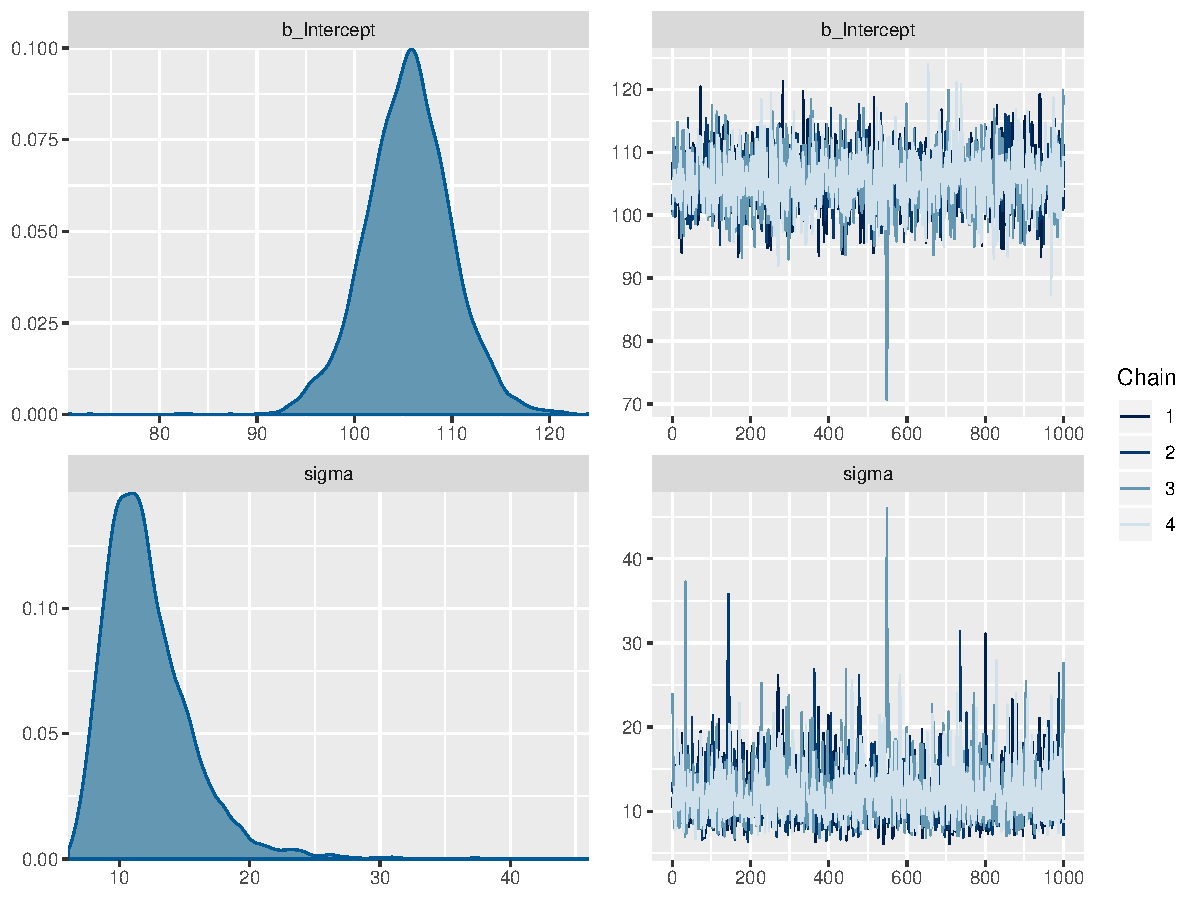
\includegraphics[width=\maxwidth]{htest-bayesex4-1} }

\caption[Posterior distributions for $\mu$ and $\sigma$ using a normal model.]{Posterior distributions for $\mu$ and $\sigma$ using a normal data model with weak priors (left panels), and convergence diagnostics for posterior sampling (right panels)}\label{fig:htest-bayesex4}
\end{figure}
\end{Schunk}

\bi
\item Normality is a strong assumption
\item Heavy tails can hurt validity of the estimate of the mean,
  uncertainty intervals, and $P$-values
\item Easy to allow for heavy tails by adding a single parameter to
  the model\footnote{One could use a data distribution with an
    additional parameter that allows for asymmetry of the
    distribution.  This is not addressed here.}
\item Assume the data come from a $t$ distribution with unknown
  degrees of freedom $\nu$
  \bi
  \item Use of $t$ for the raw data distribution should not be
    confused with the use of the same $t$ distribution for computing
    frequentist probabilities about the sample mean.
  \item John Kruschke has championed this Bayesian $t$-test approach
    in
    \href{https://cran.r-project.org/web/packages/BEST/vignettes/BEST.pdf}{BEST}
    (Bayesian Estimation Supersedes the $t$-Test)
  \ei
\item $\nu > 20 \rightarrow$ almost Gaussian
\item Have a prior for $\nu$ that is a gamma distribution with
  parameters $\alpha=2, \beta=0.1$ with $\nu$ constrained to be $> 1$
\item Prior $P(\nu > 20)$ is (in \R\ code)
  \co{pgamma(20,2,0.1,lower.tail=FALSE)} which is
  0.41.  So our prior
  probability that normality approximately holds is a little less than
  $\frac{1}{2}$. 
\ei

\begin{Schunk}
\begin{Sinput}
g <- brm(y ~ 1, family=student, prior=priormu, data=d, seed=2)
\end{Sinput}
\end{Schunk}

\begin{Schunk}
\begin{Sinput}
prior_summary(g)
\end{Sinput}
\begin{Soutput}
                prior     class coef group resp dpar nlpar bound
1     normal(150, 50) Intercept                                 
2       gamma(2, 0.1)        nu                                 
3 student_t(3, 0, 10)     sigma                                 
\end{Soutput}
\begin{Sinput}
g
\end{Sinput}
\begin{Soutput}
 Family: student 
  Links: mu = identity; sigma = identity; nu = identity 
Formula: y ~ 1 
   Data: d (Number of observations: 8) 
Samples: 4 chains, each with iter = 2000; warmup = 1000; thin = 1;
         total post-warmup samples = 4000

Population-Level Effects: 
          Estimate Est.Error l-95% CI u-95% CI Rhat Bulk_ESS Tail_ESS
Intercept   103.75      3.72    97.00   111.99 1.00     1722     1619

Family Specific Parameters: 
      Estimate Est.Error l-95% CI u-95% CI Rhat Bulk_ESS Tail_ESS
sigma     9.05      3.79     3.21    17.53 1.00     1400     1990
nu       14.30     12.87     1.47    47.98 1.00     1502     1585

Samples were drawn using sampling(NUTS). For each parameter, Eff.Sample 
is a crude measure of effective sample size, and Rhat is the potential 
scale reduction factor on split chains (at convergence, Rhat = 1).
\end{Soutput}
\begin{Sinput}
draws <- as.data.frame(g)
mu    <- draws$b_Intercept
P(mu > 110)
\end{Sinput}
\begin{Soutput}
[1] 0.054
\end{Soutput}
\begin{Sinput}
plot(g)
nu    <- draws$nu
snu   <- c(mean(nu), median(nu), pmode(nu))
ssd   <- c(sd(y), pmode(sigma), pmode(draws$sigma))
fm    <- function(x) paste(round(x, 2), collapse=', ')
\end{Sinput}
\begin{figure}[htbp]

\centerline{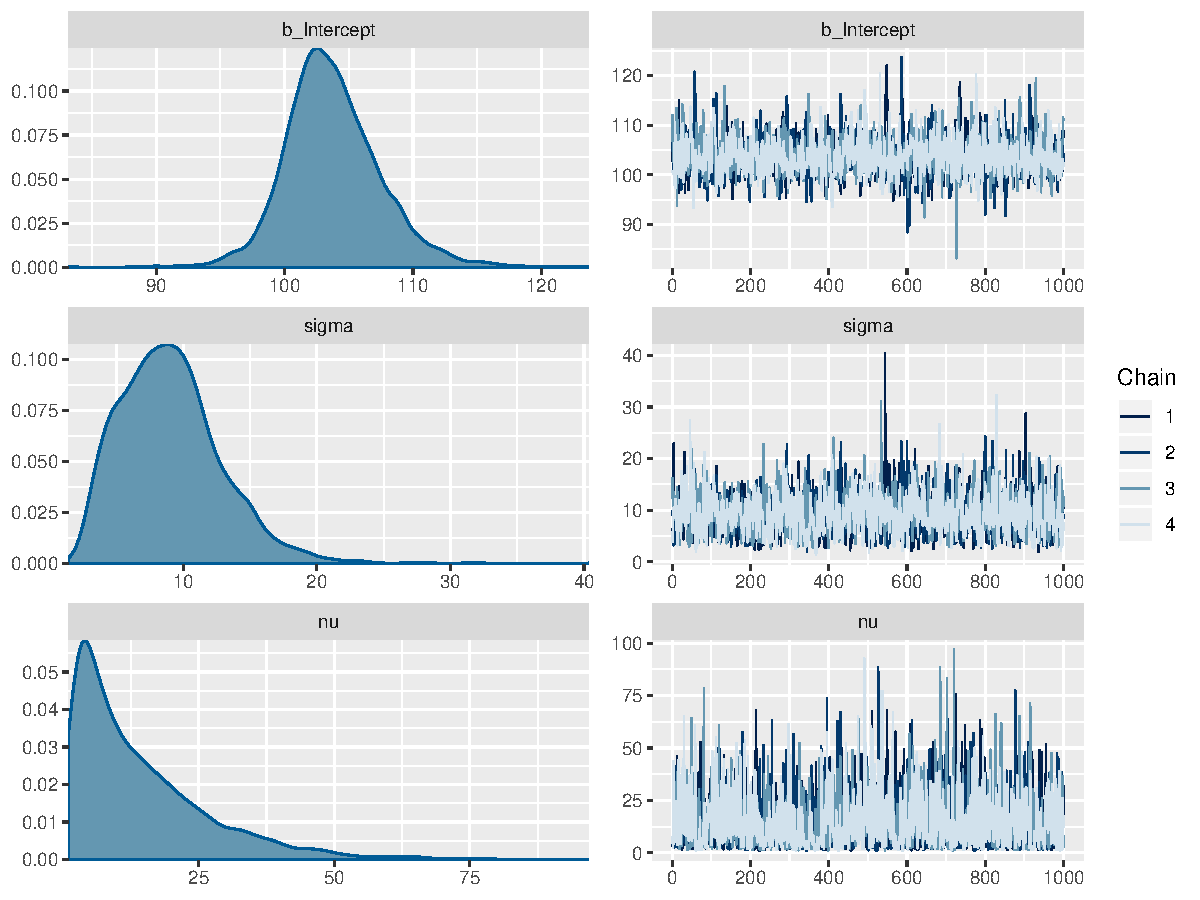
\includegraphics[width=\maxwidth]{htest-bayesext2-1} }

\caption[Posterior distributions for $\mu, \sigma, \nu$ for a $t_{\nu}$ data model]{Posterior distributions for $\mu, \sigma, \nu$ for a data model that is the $t$ distribution with $\nu$ d.f. (left panels), and convergence diagnostics (right panels)}\label{fig:htest-bayesext2}
\end{figure}
\end{Schunk}

\bi
\item Posterior means discount the high outlier a bit and shows lower
  chance of $\mu > 110$
\item The credible interval for $\mu$ is significantly smaller than
  the confidence interval due to allowance for heavy tails
\item The posterior mean, median, and mode of $\nu$
  (14.3, 10.37, 3.97) provide evidence that the 
  data come from a distribution that is heavier tailed than the
  normal.  Posterior $P(\nu > 20) = 0.25$
  which is essentially the probability of approximate normality under a $t$ data model.
\item The traditional SD estimate, posterior median SD assuming normal
  $Y$, and posterior median SD assuming $Y$ has a $t$-distribution are
  respectively 11.29, 10.98, 8.8.  The ordinary SD is giving too much
  weight to the high outlier.
\ei

This latter analysis properly penalizes for not knowing normality in
$Y$ to hold (i.e., not knowing the true value of $\nu$).

\subsubsection{Decoding the Effect of the Prior}
\bi
\item One can compute the effective number of observations added or subtracted by using, respectively, an optimistic or a skeptical prior
\item This is particularly easy when the prior is normal, the data model is normal, and the data variance is known
\item Let\\
$\mu_{0} =$ prior mean\\
$\sigma_{0} =$ prior standard deviation\\
$\overline{Y} =$ sample mean of the response variable\\
$\sigma =$ population SD of $Y$\\
$n =$ sample size for $\overline{Y}$
\item Then the posterior variance of $\mu$ is\\
$\sigma^{2}_{p} = \frac{1}{\frac{1}{\sigma^{2}_{0}} + \frac{1}{\frac{\sigma^{2}}{n}}}$
\item The posterior mean is\\
$\mu_{p} = \frac{\sigma^{2}_{p}}{\sigma^{2}_{0}} \times \mu_{0} + \frac{\sigma^{2}_{p}}{\frac{\sigma^{2}}{n}} \times \overline{Y}$
\item For a given $\overline{Y}$, sample size $n$ and posterior $P(\mu > 110)$, what sample size $m$ would yield the same posterior probability under a flat prior?
\item For a flat prior $\sigma_{0} = \infty$ so the posterior variance of $\mu$ would be $\frac{\sigma^{2}}{n}$ and the posterior mean would be $\overline{Y}$
\item Equating $P(\mu > 110)$ for the weakly informative prior at sample size $n$ to that from noninformative prior at a sample size $m$ is the same as setting $P(\mu < 110)$ to be equal
\item The probability that a Gaussian random variable with mean $a$ and standard deviation $b$ is less than 110 is $\Phi(\frac{110-a}{b})$ where $\Phi$ is the standard normal cumulative distribution function
\item Solve for $m$ for a variety of $n, \overline{Y}, \sigma$
\begin{Schunk}
\begin{Sinput}
calc <- function(n, m, ybar, sigma, mu0, sigma0, cutoff) {
  vpost1 <- 1 / ((1 / (sigma0^2)) + 1 / ((sigma^2) / n))
  mupost1 <- mu0 * vpost1 / (sigma0 ^ 2) + ybar * vpost1 / ((sigma ^ 2) / n)
  vpost2 <- (sigma ^ 2) / m
  (110 - mupost1) / sqrt(vpost1) - (110 - ybar) / sqrt(vpost2)
}

# For a given n, ybar, sigma solve for m to get equal post. prob.
m <- function(n, ybar, sigma, sigma0=50, cutoff=110) 
  round(uniroot(calc, interval=c(n / 2, 2 * n), n=n, ybar=ybar, sigma=sigma,
          mu0=150, sigma0=sigma0, cutoff=cutoff)$root, 1)
# Make sure that m=n when prior variance is huge
m(8, 100, 10, sigma0=50000)
\end{Sinput}
\begin{Soutput}
[1] 8
\end{Soutput}
\begin{Sinput}
# From here on use the original prior standard deviation of 50
# Now compute m when n=8 using our original prior assuming sigma=10 ybar=105
m(8, 105, 10)
\end{Sinput}
\begin{Soutput}
[1] 7.3
\end{Soutput}
\begin{Sinput}
# What about for two other sigmas
m(8, 105, 5)
\end{Sinput}
\begin{Soutput}
[1] 7.8
\end{Soutput}
\begin{Sinput}
m(8, 105, 15)
\end{Sinput}
\begin{Soutput}
[1] 6.6
\end{Soutput}
\begin{Sinput}
# What about two other ybar
m(8, 80, 10)
\end{Sinput}
\begin{Soutput}
[1] 7.9
\end{Soutput}
\begin{Sinput}
m(8, 120, 10)
\end{Sinput}
\begin{Soutput}
[1] 8.3
\end{Soutput}
\begin{Sinput}
# What if n were larger
m(15, 105, 10)
\end{Sinput}
\begin{Soutput}
[1] 14.3
\end{Soutput}
\begin{Sinput}
m(30, 105, 10)
\end{Sinput}
\begin{Soutput}
[1] 29.3
\end{Soutput}
\begin{Sinput}
m(300, 105, 10)
\end{Sinput}
\begin{Soutput}
[1] 299.3
\end{Soutput}
\begin{Sinput}
m(3000, 105, 10)
\end{Sinput}
\begin{Soutput}
[1] 2999.3
\end{Soutput}
\end{Schunk}
\item Typical effect of prior in this setting is like adding or dropping one observation
\item Simpler example where $\overline{Y}$ is irrelevant: $\sigma=1, \mu_{0}=0$ and posterior probability of interest is $P(\mu > 0)$
\item Vary the prior variance $\sigma^{2}_{0}$ and for each prior variance compute the prior probability that $\mu > 1$ (with prior centered at zero, lower variance $\rightarrow$ lower $P(\mu > 1)$)
\begin{Schunk}
\begin{Sinput}
z <- list()
n <- seq(1, 100, by=2)
for(v in c(.05, .1, .25, .5, 1, 4, 100))
  z[[paste0('v=', v, '     P(mu>1)=',
            format(1 - pnorm(sqrt(1 / v)), digits=3, scientific=1))]] <-
        list(x=n, y=0.5 * (n + sqrt(n^2 + 4 * n / v)) - n)

labcurve(z, pl=TRUE, xlab='Sample Size With No Skepticism',
         ylab='Extra Subjects Needed Due to Skepticism', adj=1)
\end{Sinput}
\begin{figure}[htbp]

\centerline{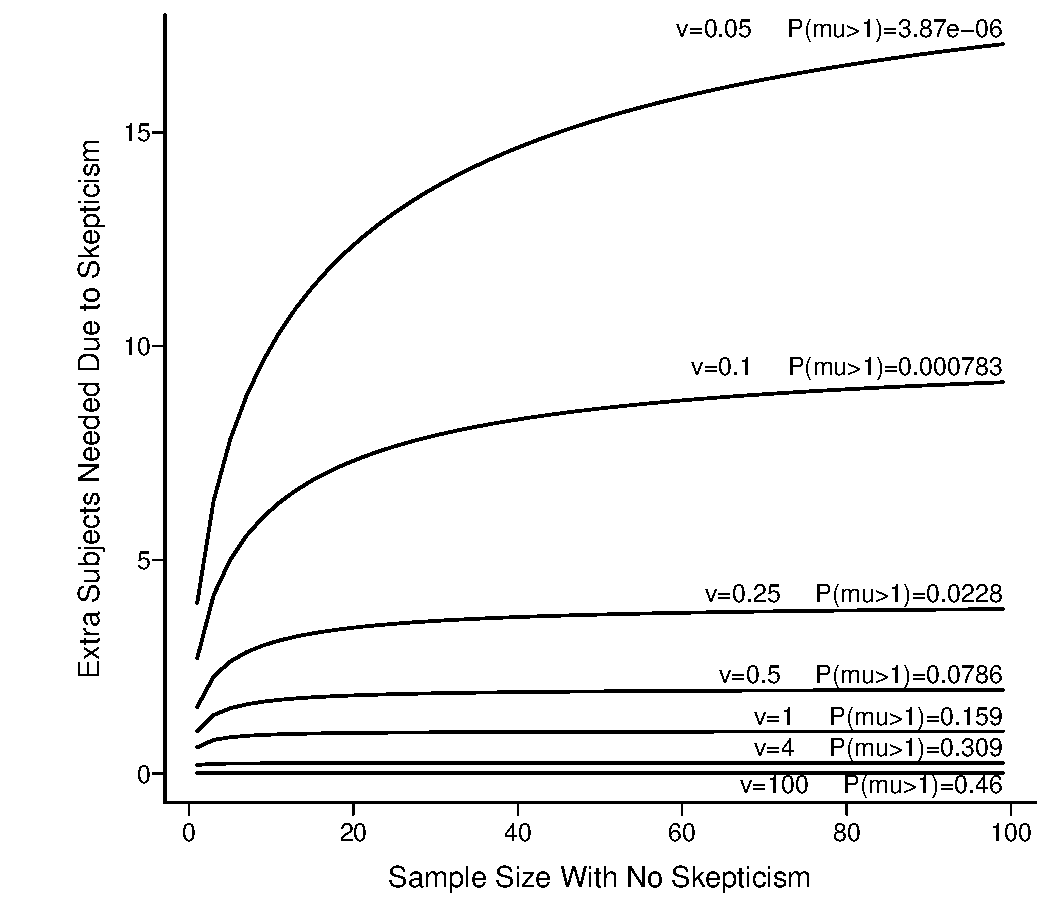
\includegraphics[width=\maxwidth]{htest-skepn-1} }

\caption[Effect of discounting by a skeptical prior]{Effect of discounting by a skeptical prior with mean zero and variance v: the increase needed in the sample size in order to achieve the same posterior probability of $\mu > 0$ as with the flat (non-informative) prior.  Prior variance v=0.05 corresponds to a very skeptical prior, given almost no chance to a large $\mu$ $(\mu > 1)$.}\label{fig:htest-skepn}
\end{figure}
\end{Schunk}

\item For typical priors the effect of skepticism is like dropping 3 observations, and this is not noticeable when $n > 20$\footnote{See \href{http://hbiostat.org/doc/bayes/course.html\#331_alternative_take_on_the_prior}{here} for the derivation.}
\item \textbf{Note}: For a specific problem one can just run the \co{brm} function again with a non-informative prior to help judge the effect of the informative prior
\ei


\subsection{Power and Sample Size} \ros{7.5-7.6}
\bi
\item Bayesian power is the probability of hitting a specified large
  posterior probability and is usually obtained by simulation
\item Frequentist power, though often arbitrary (and inviting
  optimistic single point values for an effect to detect) is easier to
  compute and will provide a decent approximation for Bayesian sample
  size calculations when the main prior is weakly informative
\item Frequentist power $\uparrow$ when
 \bi
 \item allow larger type I error ($\alpha$; trade-off between type I
   and II errors)
 \item true $\mu$ is far from $\mu_{0}$
 \item $\sigma \downarrow$
 \item $n \uparrow$
 \ei
\item Power for 2-tailed test is a function of $\mu, \mu_{0}$ and
  $\sigma$ only through  $|\mu - \mu_{0}| / \sigma$
\item Sample size to achieve $\alpha=0.05$, power $=0.9$ is approximately
\beq
n = 10.51 \left[\frac{\sigma}{\mu-\mu_{0}}\right]^{2}
\eeq
\item Some power calculators are at \url{statpages.info/#Power}
\item PS program by Dupont and Plummer \url{http://biostat.mc.vanderbilt.edu/PowerSampleSize}

\item Example: The mean forced expiratory volume (FEV) in a population of asthmatics is 2.5 liters per second and the population standard deviation is assumed to be 1.  Determine the number of subjects needed if a new drug is expected to increase FEV to 3.0 liters per second ($\alpha = .05, \beta = 0.1$)
\beqa
\mu=2.5, \mu_0=3, \sigma = 1 \\
n = 10.51 \left[\frac{1}{3-2.5}\right]^{2} = 42.04
\eeqa
  \bi
  \item \textrm{Rounding up, we need 43 subjects to have 0.9 power (42 subjects would have less than 0.9 power)}
  \ei
\ei
\begin{Schunk}
\begin{Sinput}
sigma <- 1
mu    <- 2.5
mu0   <- 3
n     <- 10.51 * (1 / (mu - mu0)) ^ 2
# General formula for approximate power of 1-sample t-test
# Approximate because it uses the normal distribution throughout,
# not the t distribution
alpha <- 0.05
power <- 0.9
delta <- mu - mu0
za    <- qnorm(1 - alpha / 2)
zb    <- qnorm(power)
n     <- ((za + zb) * sigma / delta) ^ 2
c(alpha=alpha, power=power, delta=delta, za=za, zb=zb, n=n)
\end{Sinput}
\begin{Soutput}
    alpha     power     delta        za        zb         n 
 0.050000  0.900000 -0.500000  1.959964  1.281552 42.029692 
\end{Soutput}
\end{Schunk}
A slightly more accurate estimate can be obtained using the $t$
distribution, requiring iterative calculations programmed in \R\
packages such as \co{pwr}.
\begin{Schunk}
\begin{Sinput}
# Make sure pwr package is installed
require(pwr)
\end{Sinput}
\begin{Sinput}
pwr.t.test(d = delta / sigma, power = 0.9, sig.level = 0.05, type='one.sample')
\end{Sinput}
\begin{Soutput}

     One-sample t test power calculation 

              n = 43.99548
              d = 0.5
      sig.level = 0.05
          power = 0.9
    alternative = two.sided
\end{Soutput}
\end{Schunk}

\subsection{Confidence Interval} \ros{R7.7}\altman{28-29}\abd{6.6}
A 2-sided $1-\alpha$ confidence interval for $\mu$ under normality for $Y$ is
\beq
\bar{x} \pm t_{n-1,1-\alpha/2} \times {se}
\eeq
The $t$ constant is the $1-\alpha/2$ level critical value from the
$t$-distribution with $n-1$ degrees of freedom.  For large $n$ it
equals 1.96 when $\alpha=0.05$.

An incorrect but common way to interpret this is that we are 0.95
confident that the 
unknown $\mu$ lies in the above interval.  The exact way to say it is
that if we were able to repeat the same experiment 1000 times and
compute a fresh confidence interval for $\mu$ from each sample, we
expect 950 of the samples to actually contain $\mu$.  The confidence
level is about the procedure used to derive the interval, not about
any one interval.  Difficulties in
providing exact but still useful interpretations of confidence intervals has driven
many people to Bayesian statistics.

The 2-sided $1-\alpha$ CL includes $\mu_{0}$ if and only if a test of $H_{0}:
\mu=\mu_{0}$ is not rejected at the $\alpha$ level in a 2-tailed test.
\bi
\item If a 0.95 CL does not contain zero, we can reject $H_0: \mu = 0$ at the $\alpha = 0.05$ significance level
\ei

$1 - \alpha$ is called the \emph{confidence level} or \emph{confidence
  coefficient}, but it is better to refer to \emph{compatibility}

\subsection{Sample Size for a Given Precision} \altman{139-148}\abd{14.7}
There are many reasons for preferring to run estimation studies
instead of hypothesis testing studies.  A null hypothesis may be
irrelevant, and when there is adequate precision one can learn from a
study regardless of the magnitude of a $P$-value.  A nearly universal
property of precision estimates is that, all other things being equal,
increasing the sample size by a factor of four improves the precision
by a factor of two.
\bi
\item May want to estimate $\mu$ to within a margin of error of $\pm
  \delta$ with 0.95 confidence\footnote{Adcock~\cite{adc97sam}
    presents both frequentist and Bayesian methods and for precision
    emphasizes solving for $n$ such that the probability of being
    within $\epsilon$ of the true value is controlled, as opposed to
    using confidence interval widths explicitly.}
\item ``0.95 confident'' that a confidence interval includes the true
  value of $\mu$
\item If $\sigma$ were known but we still used the $t$ distribution in
  the formula for the interval, the confidence interval would be
  $\bar{x}\pm \delta$ where
\beq
\delta = \frac{t_{n-1,1-\alpha/2}\sigma}{\sqrt{n}}
\eeq
\item Solving for $n$ we get
\beq
n = \left[\frac{t_{n-1,1-\alpha/2} \sigma}{\delta}\right]^{2}
\eeq
\item If $n$ is large enough and $\alpha=0.05$, required
  $n=3.84[\frac{\sigma}{\delta}]^{2}$
\item Example: if want to be able to nail down $\mu$ to within $\pm
  1$mmHg when the patient to patient standard deviation in blood
  pressure is 10mmHg, $n = 384$
\begin{Schunk}
\begin{Sinput}
sigma <- 10
delta <- 1
3.84 * (sigma / delta) ^ 2
\end{Sinput}
\begin{Soutput}
[1] 384
\end{Soutput}
\end{Schunk}
\item Advantages of planning for precision rather than
  power\footnote{See Borenstein M: \emph{J Clin Epi} 1994;
    47:1277-1285.}
 \bi
 \item do not need to select a single effect to detect
 \item many studies are powered to detect a miracle and nothing less;
   if a miracle doesn't happen, the study provides \textbf{no} information
 \item planning on the basis of precision will allow the resulting
   study to be interpreted if the $P$-value is 
   large, because the confidence interval will not be so wide as to
   include both clinically significant improvement and clinically
   significant worsening
 \ei
\ei

\section{One Sample Method for a Probability} \ros{7.10}\altman{45-56}\abd{7}
\subsection{Frequentist Methods}
\bi
\item Estimate a population probability $p$ with a sample estimate
  $\hat{p}$
\item Data: $s$ ``successes'' out of $n$ trials
\item Maximum likelihood estimate of $p$ is $\hat{p} = \frac{s}{n}$ (value of
  $p$ making the data most likely to have been observed) = Bayesian
  posterior mode  under a flat prior
\item Approximate 2-sided test of $H_{0}: p=p_{0}$ obtained by
  computing a $z$ statistic
\item A $z$-test is a test assuming that the \emph{statistic} has
  a normal distribution; it is a $t$-test with infinite ($\infty$) d.f.
\beq
z = \frac{\hat{p} - p_{0}}{\sqrt{p_{0}(1-p_{0})/n}}
\eeq
\item The $z$-test follows the same general form as the $t$-test
\beq
z = \frac{\textrm{estimate - hypothesized value}}{\textrm{standard deviation
  of numerator}}
\eeq
\item Example: $n=10$ tosses of a coin, 8 heads; $H_{0}$: coin is fair
  ($p = p_{0}=\frac{1}{2}$)
\beq
z = \frac{.8 - .5}{\sqrt{(\frac{1}{2})(\frac{1}{2})/10}} = 1.897
\eeq
\item $P\textrm{-value} = 2 \times$ area under a normal curve to the right of $1.897 =
  2 \times 0.0289 = 0.058$ (this is also the area under the normal
  curve to the right of $1.897$ + the area to the left of $-1.897$)
\begin{Schunk}
\begin{Sinput}
p  <- 0.8
p0 <- 0.5
n  <- 10
z  <- (p - p0) / sqrt(p0 * (1 - p0) / n)
c(z=z, Pvalue=2 * pnorm(-abs(z)))
\end{Sinput}
\begin{Soutput}
         z     Pvalue 
1.89736660 0.05777957 
\end{Soutput}
\end{Schunk}
\item Approximate probability of getting 8 or more or 2 or fewer heads
  if the coin is fair is 0.058.  \textbf{This is indirect evidence for
    fairness, is not the probability the null hypothesis is true, and
    invites the ``absence of evidence is not evidence of absence'' error.}
\item Use exact methods if $p$ or $n$ is small
\begin{Schunk}
\begin{Sinput}
# Pr(X >= 8) = 1 - Pr(X < 8) = 1 - Pr(X <= 7)
pbinom(2, 10, 0.5) + 1 - pbinom(7, 10, 0.5)
\end{Sinput}
\begin{Soutput}
[1] 0.109375
\end{Soutput}
\begin{Sinput}
# Also compute as the probability of getting 0, 1, 2, 8, 9, 10 heads
sum(dbinom(c(0, 1, 2, 8, 9, 10), 10, 0.5))
\end{Sinput}
\begin{Soutput}
[1] 0.109375
\end{Soutput}
\end{Schunk}
\item Confidence interval for $p$
  \bi
  \item
    \href{https://en.wikipedia.org/wiki/Binomial_proportion_confidence_interval}{Wilson's
      method} without continuity correction is recommended
  \item for 8 of 10 heads here is the Wilson interval in addition to
    the exact binomial and normal approximation.  The Wilson interval
    is the most accurate of the three.
  \ei
  
\begin{Schunk}
\begin{Sinput}
binconf(8, 10, method='all')
\end{Sinput}
\begin{Soutput}
           PointEst     Lower     Upper
Exact           0.8 0.4439045 0.9747893
Wilson          0.8 0.4901625 0.9433178
Asymptotic      0.8 0.5520820 1.0479180
\end{Soutput}
\end{Schunk}
\ei

\subsection{Bayesian}
\bi
\item The single unknown probability $p$ for binary $Y$-case is a
  situation where there is a top choice for prior distributions
\item Number of events follows a binomial distribution with parameters
  $p, n$
\item The beta distribution is for a variable having a range of $[0,
  1]$, has two parameters $\alpha, \beta$ for
  flexibility, and is \emph{conjugate} to the binomial distribution
  \bi
  \item The posterior distribution is simple: another beta distribution
  \ei
\item The mean of a beta-distributed variable is $\frac{\alpha}{\alpha
    + \beta}$ and its standard deviation is\\
  $\sqrt{\frac{\alpha\beta}{\alpha+\beta+1}} / (\alpha + \beta)$
\item Using a beta prior is equivalent to adding $\alpha$ successes
  and $\beta$ failures to the data
\item Posterior distribution of $p$ is beta$(s + \alpha, n - s + \beta)$
\item A uniform prior sets $\alpha = \beta = 1$
\item In general an intuitive way to set the prior is to preset the
  mean then solve for the parameters that force $P(p > c) = a$ for
  given $c$ and $a$
\item For the 10 coin toss example let's set the prior mean of
  P$($heads$)=\frac{1}{2}$ and $P(p > 0.8) = 0.05$, i.e. only a 0.05
  chance that the probability of heads exceeds 0.8.  Here are $\alpha$
  and $\beta$ satisfying these requirements:
\begin{Schunk}
\begin{Sinput}
# alpha/(alpha + beta) = 0.5 -> alpha=beta
alphas <- seq(0, 20, length=100000)
exceedanceProb <- 1 - pbeta(0.8, alphas, alphas)
alpha <- alphas[which.min(abs(exceedanceProb - 0.05))]
beta  <- alpha
alpha.post <- 8 + alpha
beta.post  <- 10 - 8 + beta
\end{Sinput}
\end{Schunk}
\item The solution is $\alpha=\beta=3.26$
\item With the data $s=8$ out of $n=10$ the posterior distribution is
  beta(11.26, 5.26)

\begin{Schunk}
\begin{Sinput}
p <- seq(0, 1, length=300)
prior <- dbeta(p, alpha, beta)
post  <- dbeta(p, alpha.post, beta.post)
curves <- list(Prior=list(x=p, y=prior),
               Posterior=list(x=p, y=post))
labcurve(curves, pl=TRUE, xlab='p', ylab='Probability Density')
\end{Sinput}
\begin{figure}[htbp]

\centerline{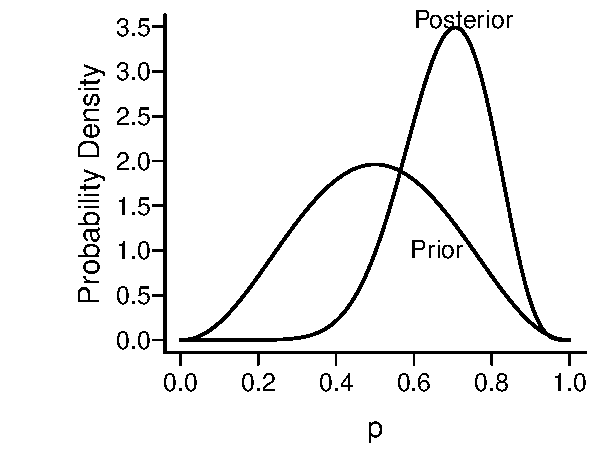
\includegraphics[width=\maxwidth]{htest-plotbetapost-1} }

\caption[Prior and posterior distributions for unknown probability of heads]{Prior and posterior distribution for the unknown probability of heads.  The posterior is based on tossing 8 heads out of 10 tries.}\label{fig:htest-plotbetapost}
\end{figure}
\end{Schunk}

\item From the posterior distribution we can get the credible interval, the
probability that the probability of heads exceeds $\frac{1}{2}$, and
the probability that the probability of heads is within $\pm
0.05$ of fairness:
\begin{Schunk}
\begin{Sinput}
qbeta(c(.025, .975), alpha.post, beta.post)
\end{Sinput}
\begin{Soutput}
[1] 0.4464199 0.8751905
\end{Soutput}
\begin{Sinput}
1 - pbeta(0.5, alpha.post, beta.post)
\end{Sinput}
\begin{Soutput}
[1] 0.9374297
\end{Soutput}
\begin{Sinput}
pbeta(0.55, alpha.post, beta.post) - pbeta(0.45, alpha.post, beta.post)
\end{Sinput}
\begin{Soutput}
[1] 0.100748
\end{Soutput}
\end{Schunk}

\item Unlike the frequentist analysis, these are direct measures that are
easier to interpret
\item Instead of just providing evidence against a
straw-man assertion, Bayesian posterior probabilities measure evidence
in favor (as well as against) all possible assertions
\ei

\subsection{Power and Sample Size}
\bi
\item Power $\uparrow$ as $n \uparrow$, $p$ departs from $p_{0}$, or
  $p_{0}$ departs from $\frac{1}{2}$
\item $n \downarrow$ as required power $\downarrow$ or $p$ departs
  from $p_{0}$
\ei

\subsection{Sample Size for Given Precision}\alabel{sec:htest-p-n}
\bi
\item Approximate 0.95 CL: $\hat{p} \pm 1.96
  \sqrt{\hat{p}(1-\hat{p})/n}$
\item Assuming $p$ is between 0.3 and 0.8, it would not be far off to
  use the worst case standard error $\sqrt{1/(4n)}$ when planning
\item $n$ to achieve a margin of error $\delta$ in estimating $p$: 
\beq
n = \frac{1}{4}\left[\frac{1.96}{\delta}\right]^{2} = \frac{0.96}{\delta^{2}}
\eeq
\item Example: $\delta=.1 \rightarrow n=96$ to achieve a margin of error of
  $\pm 0.1$ with 0.95 confidence
\ei
\begin{Schunk}
\begin{Sinput}
nprec <- function(delta) round(0.25 * (qnorm(0.975) / delta) ^ 2)
nprec(0.1)
\end{Sinput}
\begin{Soutput}
[1] 96
\end{Soutput}
\end{Schunk}

To achieve a margin of error of $\pm 0.05$ even in the worst case where
$p=0.5$ one needs $n=384$.

For Bayesian precision calculations we can solve $n$ that achieves a
given width of, say, a 0.95 credible interval:

\bi
\item Use a flat beta prior, i.e., with $\alpha=\beta=1$
\item Posterior distribution for $p$ is $\textrm{beta}(s + 1, n - s + 1)$
\item Compute CI half-widths for varying $n$ for selected values of $s$
\begin{Schunk}
\begin{Sinput}
n <- seq(10, 400, by=5)
k <- c(1/8, 1/4, 1/2, 3/4, 7/8)
ck <- paste0('s=', c('1/8', '1/4', '1/2', '3/4', '7/8'), ' n')
r <- list()
for(i in 1 : 5) {
   ciu <- qbeta(0.975, k[i] * n + 1, n - k[i] * n + 1)
   cil <- qbeta(0.025, k[i] * n + 1, n - k[i] * n + 1)
   r[[ck[i]]] <- list(x=n, y=(ciu - cil) / 2)
}
labcurve(r, xlab='n', ylab='Precision', col=1:5, pl=TRUE)
abline(h=c(0.05, 0.1), col=gray(0.9))
\end{Sinput}
\begin{figure}[htbp]

\centerline{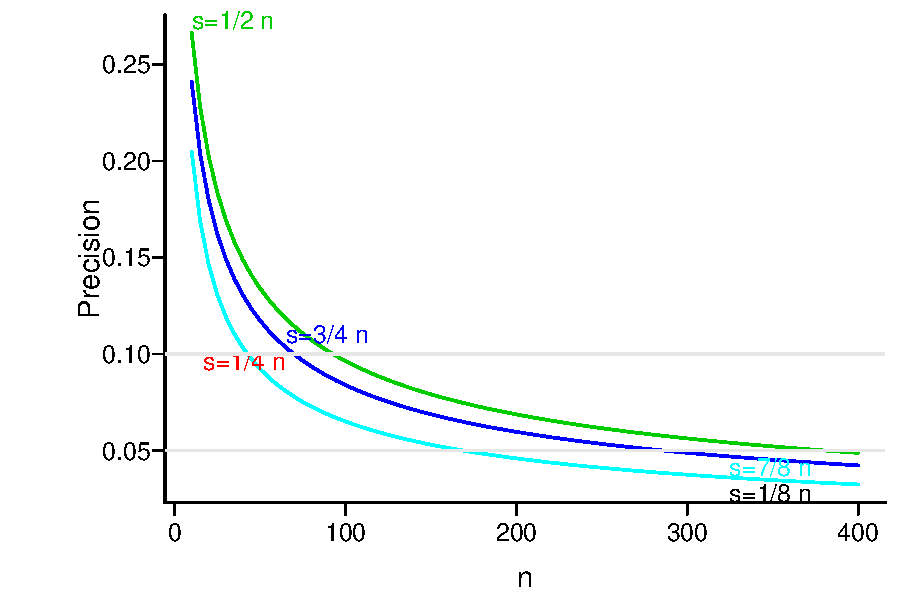
\includegraphics[width=\maxwidth]{htest-pprecb-1} }

\caption[Half-widths of 0.95 credible intervals for $p$ using a flat prior]{Half-widths of 0.95 credible intervals for $p$ using a flat prior}\label{fig:htest-pprecb}
\end{figure}
\end{Schunk}
\item As with confidence intervals, precision is worst when
  $\frac{1}{2}$ of observations are successes, so often best to plan
  on worst case
\item Same sample size needed as with frequentist (since prior is flat)  
\item Easy to modify for other priors
\ei

To put this in the context of relative errors, suppose that one wants
to estimate the odds that an event will occur, to within a certain
multiplicative margin of error (MMOE) with 0.95 confidence using
frequentist methods.  What is
the MMOE as a function of the unknown $p$ when $n=384$?  The standard
error of the log odds is approximately $\sqrt{\frac{1}{n p (1 - p)}}$,
and the half-width of a 0.95 confidence interval for the log odds is
approximately 1.96 times that.  Fix $n=384$ and vary $p$ to get the
MMOE that is associated with the same sample size as a universal
absolute margin of error of 0.05.

\begin{Schunk}
\begin{Sinput}
p <- seq(0.01, 0.99, length=200)
mmoe <- exp(1.96 / sqrt(384 * p * (1 - p)))
plot(p, mmoe, type='l', xlab='Unknown Probability p', ylab='MMOE')
minor.tick()
\end{Sinput}
\begin{figure}[htbp]

\centerline{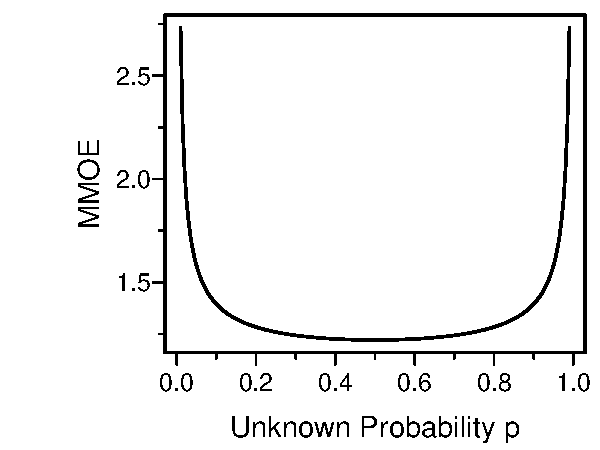
\includegraphics[width=\maxwidth]{htest-moeor-1} }

\caption[Multiplicative margin of error in estimating odds when $n=384$ and the margin of error in estimating the absolute probability is $\leq 0.05$]{Multiplicative margin of error in estimating odds when $n=384$ and the margin of error in estimating the absolute probability is $\leq 0.05$.}\label{fig:htest-moeor}
\end{figure}
\end{Schunk}

\section{Paired Data and One-Sample Tests}  \altman{31-32}\abd{11}
\bi
\item To investigate the relationship between smoking and bone mineral
  density, Rosner presented a paired analysis in which each person had
  a nearly perfect control which was his or her twin
\item Data were normalized by dividing differences by the mean density
  in the twin pair (need to check if this normalization worked)
\item \textbf{Note}: It is almost never appropriate to compute mean percent change (a 100\% increase is balanced by a 50\% decrease) but we plunge ahead anyway
\item Computed density in heavier smoking twin minus density in
  lighter smoking one
\item Mean difference was $-5\%$ with se=$2.0\%$ on $n=41$
\item The $t$ statistic we've been using works here, once within-pair
  differences are formed
\item $H_{0}:$ mean difference between twins is zero ($\mu_{0} = 0$)
\beqa
t_{40} = \frac{\bar{x} - \mu_{0}}{se} = -2.5 \\
P = 0.0166
\eeqa
\ei
\begin{Schunk}
\begin{Sinput}
xbar  <- -5
se    <- 2
n     <- 41
mu0   <- 0
tstat <- (xbar - mu0) /se
pval  <- 2 * (1 - pt(abs(tstat), n - 1))
c(tstat=tstat, Pvalue=pval)
\end{Sinput}
\begin{Soutput}
      tstat      Pvalue 
-2.50000000  0.01662035 
\end{Soutput}
\end{Schunk}

\section{Two Sample Test for Means} \ros{8}\katz{5.5}\altman{28-35}\abd{12}\bmovie{6}\ddisc{6}
\bi
\item Two groups of different patients (unpaired data)
\item Much more common than one-sample tests
\item As before we are dealing for now with parametric tests assuming
  the raw data arise from a normal distribution
\item We assume for now that the two groups have the same
  spread or variability in the distributions of
  responses\footnote{Rosner covers the unequal variance case very
    well.  As nonparametric tests have advantages for comparing two
    groups and are less sensitive to the equal spread assumption, we
    will not cover the unequal variance case here.}
\ei

\subsection{Frequentist $t$-Test}
\bi
\item Test whether population 1 has the same mean as population 2
\item Example: pop.\ 1=all patients with a certain disease if given
  the new drug, pop.\ 2=standard drug
\item $H_{0}: \mu_{1}=\mu_{2}$ (this can be generalized to test
  $\mu_{1}=\mu_{2}+\delta$, i.e., $\mu_{1}-\mu_{2}=\delta$).  The
  \emph{quantity of interest} or \emph{QOI} is $\mu_{1}-\mu_{2}$
\item 2 samples, of sizes $n_{1}$ and $n_{2}$ from two populations
\item Two-sample (unpaired) $t$-test assuming normality and equal
variances---recall that if we are testing against an $H_0$ of
\textbf{no effect}, the form of the $t$ test is
\beq
t =
\frac{\mathrm{point~estimate~of~QOI}}{\mathrm{se~of~numerator}}
\eeq
\item Point estimate QOI is $\bar{x}_{1} - \bar{x}_{2}$
\item As with 1-sample $t$-test the difference in the numerator is judged with respect to the precision in the denominator (combination of sample size and subject-to-subject variability); like a signal:noise ratio
\item Variance of the sum or difference of two independent means is
  the sum of the variance of the individual means
\item This is $\frac{\sigma^{2}}{n_{1}} + \frac{\sigma^{2}}{n_{2}} =
  \sigma^{2}[\frac{1}{n_{1}} + \frac{1}{n_{2}}]$
\item Need to estimate the single $\sigma^{2}$ from the two samples
\item We use a weighted average of the two sample variances:
\beq
s^{2} = \frac{(n_{1}-1)s^{2}_{1} + (n_{2}-1)s^{2}_{2}}{n_{1}+n_{2}-2}
\eeq
\item True standard error of the difference in sample means: $\sigma
  \sqrt{\frac{1}{n_{1}} + \frac{1}{n_{2}}}$
\item Estimate: $s \sqrt{\frac{1}{n_{1}} + \frac{1}{n_{2}}}$, so
\beq
t = \frac{\bar{x}_{1} - \bar{x}_{2}}{s \sqrt{\frac{1}{n_{1}} + \frac{1}{n_{2}}}}
\eeq
\item d.f.\ is the sum of the individual d.f., $n_{1}+n_{2}-2$, where
  the $-2$ is from our having to estimate the center of two
  distributions
\item If $H_{0}$ is true $t$ has the $t_{n_{1}+n_{2}-2}$ distribution
\item To get a 2-tailed $P$-value we compute the probability that a
  value from such a distribution is farther out in the tails of the
  distribution than the observed $t$ value is (we ignore the sign of
  $t$ for a 2-tailed test)
\item Example: $n_{1}=8, n_{2}=21, s_{1}=15.34, s_{2}=18.23,
  \bar{x}_{1}=132.86, \bar{x}_{2}=127.44$
\beqa
s^{2} &=& \frac{7(15.34)^{2}+20(18.23)^{2}}{7+20} = 307.18 \\
s     &=& \sqrt{307.18} = 17.527 \\
se    &=& 17.527 \sqrt{\frac{1}{8}+\frac{1}{21}} = 7.282 \\
t     &=& \frac{5.42}{7.282} = 0.74
\eeqa
on 27 d.f.
\item $P = 0.463$ (see \R\ code below)
\item Chance of getting a difference in means as larger or larger than
  5.42 if the two populations really have the same means is 0.463
\item $\rightarrow$ little evidence for concluding the population
  means are different
\ei
\begin{Schunk}
\begin{Sinput}
n1    <- 8;         n2 <- 21
xbar1 <- 132.86; xbar2 <- 127.44
s1    <- 15.34;     s2 <- 18.23
s     <- sqrt(((n1 - 1) * s1 ^ 2 + (n2 - 1) * s2 ^ 2) / (n1 + n2 - 2))
se    <- s * sqrt(1 / n1 + 1 / n2)
tstat <- (xbar1 - xbar2) / se
pval  <- 2 * (pt(- abs(tstat), n1 + n2 - 2))
c(s=s, se=se, tstat=tstat, Pvalue=pval)
\end{Sinput}
\begin{Soutput}
         s         se      tstat     Pvalue 
17.5265589  7.2818380  0.7443176  0.4631137 
\end{Soutput}
\end{Schunk}

\subsection{Confidence Interval}  \ros{8.5}\altman{28-35}
Assuming equal variances

\beq
\bar{x}_{1}-\bar{x}_{2} \pm t_{n_{1}+n_{2}-2,1-\alpha/2} \times s \times
\sqrt{\frac{1}{n_{1}} + \frac{1}{n_{2}}}
\eeq
is a $1-\alpha$ CL for $\mu_{1}-\mu_{2}$, where $s$ is the pooled
estimate of $\sigma$, i.e., $s \sqrt{\ldots}$ is the estimate of the
standard error of $\bar{x}_{1}-\bar{x}_{2}$

\subsection{Bayesian $t$-Test}
\bi
\item As with one-sample Bayesian $t$-test we relax the normality assumption by using a $t$ distribution for the raw data (more robust analysis)
\item A linear model for the two-sample $t$ test is\\
  $Y = \mu_{0} + \delta[\textrm{group B}] + \epsilon$\\
  where $\mu_{0}$ (the intercept) is the unknown group A mean, $\delta$ is the B-A difference in means, and $\epsilon$ is the irreducible residual (assuming we have no covariates to adjust for)
\item Assume:
 \bi
 \item $\epsilon$ has a $t$-distribution with $\nu$ d.f.
 \item $\nu$ has a prior that allows the data distribution to be anywhere from heavy-tailed to normal
 \item $\mu_{0}$ has a fairly wide prior distribution (no prior knowledge may be encoded by using a flat prior)
 \item $\delta$ has either a prior that is informed by prior reliable research or biological knowledge, or has a skeptical prior
 \item residual variance $\sigma^2$ is allowed to be different for groups A and B, with a normal prior on the log of the variance ratio that favors equal variance but allows the ratio to be different from 1 (but not arbitrarily different)
 \ei
Note: by specifying independent priors for $\mu_{0}$ and $\delta$ we
 \bi
 \item induce correlations in priors for the two means
 \item assume we know more about $\delta$ than about the individual true per-group means 
 \ei
\ei
To specify the SD for the prior for the log variance ratio:
\bi
\item Let $r$ be unknown ratio of variances
\item Assume $P(r > 1.5) = P(r < \frac{1}{1.5}) = \gamma$
\item The required SD is $\frac{\log{1.5}}{-\Phi^{-1}(\gamma)}$
\item For $\gamma=0.15$ the required SD is:
\begin{Schunk}
\begin{Sinput}
log(1.5) / -qnorm(0.15)
\end{Sinput}
\begin{Soutput}
[1] 0.3912119
\end{Soutput}
\end{Schunk}

\ei

We are assuming a mean of zero for $\log(r)$ so we favor $r=1$ and give equal chances to ratios smaller or larger than 1.
\subsection{Power and Sample Size}
\bi
\item Consider the frequentist model
\item Power increases when
 \bi
 \item $\Delta = |\mu_{1}-\mu_{2}| \uparrow$
 \item $n_{1} \uparrow$ or $n_{2} \uparrow$
 \item $n_{1}$ and $n_{2}$ are close
 \item $\sigma \downarrow$
 \item $\alpha \uparrow$
 \ei
\item Power depends on $n_{1}, n_{2}, \mu_{1}, \mu_{2}, \sigma$
  approximately through 
\beq
\frac{\Delta}{\sigma \sqrt{\frac{1}{n_{1}}+\frac{1}{n_{2}}}}
\eeq
\item Note that when computing power using a program that asks for
  $\mu_{1}$ and $\mu_{2}$ you can just enter 0 for $\mu_{1}$ and enter
  $\Delta$ for $\mu_{2}$, as only the difference matters
\item Often we estimate $\sigma$ from pilot data, and to be honest we
  should make adjustments for having to estimate $\sigma$ although we
  usually run out of gas at this point (Bayes would help)
\item Use the \R\ \co{pwr} package, or the power calculator at
  \url{statpages.org/#Power} or PS 
\item Example: \\
 Get a pooled estimate of $\sigma$ using $s$ above (17.52656) \\
% $\sqrt{\frac{15.34^{2}+18.23^{2}}{2}} = 
% 16.847$ when
 Use $\Delta=5, n_{1}=n_{2}=100, \alpha=0.05$
\begin{Schunk}
\begin{Sinput}
delta <- 5
require(pwr)
pwr.t2n.test(n1=100, n2=100, d=delta / s, sig.level = 0.05)
\end{Sinput}
\begin{Soutput}

     t test power calculation 

             n1 = 100
             n2 = 100
              d = 0.2852813
      sig.level = 0.05
          power = 0.5189751
    alternative = two.sided
\end{Soutput}
\end{Schunk}
\item Sample size depends on $k = \frac{n_{2}}{n_{1}}$, $\Delta$, power,
  and $\alpha$
\item Sample size $\downarrow$ when
 \bi
 \item $\Delta \uparrow$
 \item $k \rightarrow 1.0$
 \item $\sigma \downarrow$
 \item $\alpha \uparrow$
 \item required power $\downarrow$
 \ei
\item An approximate formula for required sample sizes to achieve
  power $=0.9$ with $\alpha=0.05$ is
\beqa
n_{1} &=& \frac{10.51 \sigma^{2} (1+\frac{1}{k})}{\Delta^{2}} \\
n_{2} &=& \frac{10.51 \sigma^{2} (1+k)}{\Delta^{2}}
\eeqa
%\item Example using web page: \\
%Does not allow unequal $n_1$ and $n_2$; use power=0.8, $\alpha=0.05,
%\mu_{1}=132.86, \mu_{2}=127.44, \sigma=16.847$
%\item Result is 153 in each group (total=306) vs.\ Rosner's
%  $n_{1}=108, n_{2}=216$, total=324.  The price of having unequal
%  sample sizes was 18 extra patients.
\item Exact calculations assuming normality
\begin{Schunk}
\begin{Sinput}
pwr.t.test(d = delta / s, sig.level = 0.05, power = 0.8)
\end{Sinput}
\begin{Soutput}

     Two-sample t test power calculation 

              n = 193.8463
              d = 0.2852813
      sig.level = 0.05
          power = 0.8
    alternative = two.sided

NOTE: n is number in *each* group
\end{Soutput}
\end{Schunk}
\item If used same total sample size of 388 but did a 2:1
  randomization ratio to get 129 in one group and 259 in the other,
  the power is less
\begin{Schunk}
\begin{Sinput}
pwr.t2n.test(n1 = 129, n2 = 259, d = delta / s, sig.level = 0.05)
\end{Sinput}
\begin{Soutput}

     t test power calculation 

             n1 = 129
             n2 = 259
              d = 0.2852813
      sig.level = 0.05
          power = 0.7519836
    alternative = two.sided
\end{Soutput}
\end{Schunk}
\ei

What is the difference in means that would yield a 2-sided $P$-value
of exactly 0.05 for a two-sample $t$-test with normality and equal
variances when the sample sizes are both equal to $\frac{n}{2}$?  We
solve for $\hat{\Delta} = \bar{x}_{1} - \bar{x}_{2}$ such 
that $t_{n-2,1-\alpha/2} = \frac{\hat{\Delta}}{2s/\sqrt{n}}$, giving
\beq
\hat{\Delta} = \frac{2 \times t_{n-2,1-\alpha/2} \times s}{\sqrt{n}}
\eeq
For total sample sizes of 10, 50, and 100, the ``magic'' values of the
observed difference are the following multiples of the observed
standard deviation $s$:
\begin{Schunk}
\begin{Sinput}
n <- c(10, 50, 100)
tcrit <- qt(0.975, n-2)
2 * tcrit / sqrt(n)
\end{Sinput}
\begin{Soutput}
[1] 1.4584451 0.5686934 0.3968935
\end{Soutput}
\end{Schunk}
Note that these thresholds are independent of the power and the effect
size used in the power calculation.


\subsection{Sample Size for a Given Precision}\label{sec:htest-t2-moe}
To design a study that will nail down the estimate of $\mu_{1}-\mu_{2}$
to within $\pm \delta$ with $1-\alpha$ confidence when $n_{1}=n_{2}=n$, and
when $n$ is large enough so that the critical value
$t_{2n-2,1-\alpha/2}$ may be approximated by the critical value from
the normal distribution, say $z$ ($z=1.96$ when $\alpha=0.05$):
\beq
n = 2\left[\frac{z \sigma}{\delta}\right]^{2}
\eeq
When $\alpha=0.05$, $n = 7.68 [\frac{\sigma}{\delta}]^{2}$

\subsection{Equating Margin of Error to Detectable Difference}
Suppose that a two-arm study is designed to detect a difference $\Delta$ in two
means with power 0.9 at the $\alpha=0.05$ level.  For large enough
sample sizes, the margin of error for estimating the true difference
in means for that study will be $\delta =
\Delta\sqrt{\frac{7.68}{21.02}} = 0.604\Delta$.

\subsection{Checking Assumptions of the $t$-test}
\bi
\item Comprehensive assessment of all assumptions except independence of observations:
 \bi
 \item Compute the two empirical cumulative distribution functions
 \item Transform each using the inverse normal $z$ transformation
 \item See of both curves are linear (checks normality assumption) and parallel (equal variance assumption)\footnote{There are formal tests of normality but in smaller samples these have insufficient power to detect important non-normality.}
 \ei
\item Box plot (one box for each of 2 groups): look for equal spread
  (IQR)
\item Informally compare $s_{1}$ and $s_{2}$\footnote{Rosner 8.6 shows how to
  make formal comparisons, but beware that the variance ratio test
  depends on normality, and it may not have sufficient power to detect
  important differences in variances.}
\item With the Bayesian $t$-test the only important assumption to check is symmetry of the data distribution\footnote{Since we are allowing for heavier tails than the Gaussian distribution by using a $t$ distribution for the raw data}
\ei

\section{Comprehensive Example: Two sample $t$-test}

\subsection{Study Description}
From \href{http://learntech.uwe.ac.uk/da/Default.aspx?pageid=1438}{bit.ly/data-t2}

\bi
\item Assess the effect of caffeine (vs.\ placebo) on muscle
  metabolism, measured by the respiratory exchange ratio (RER; ratio
  of CO$_{2}$ produced to O$_{2}$ consumed)
\item Treatment was randomized to 18 subjects; parallel group RCT
\item Goal: study effect of caffeine on RER
\item Must take log of RER to have a symmetric measure
  \bi
  \item $\mu_0$ = mean log RER for placebo
  \item $\mu_1$ = mean log RER for caffeine
  \item Fold-change effect: $\exp(\mu_1 - \mu_0)$
  \item Estimate $ \mu_1 - \mu_0$
  \item $H_0: \mu_0 = \mu_1$
  \item $H_1: \mu_0 \neq \mu_1$
  \ei
  \item Note: a good statistician will take such ratios with a grain of salt; need to verify that the meaning of the ratio is independent of O$_{2}$
\ei

\subsection{Power and Sample Size}

\bi
\item Suppose that a pilot study or previous published research
  estimated $\sigma = 0.1$ for log RER
\item Effect size $\Delta$ is on the log RER scale
\item Anti-log to get effect in terms of fold change
\item Determine the number of subjects needed (in each group) for several value of effect size $\Delta$ ($\Delta = |\mu_1 - \mu_0|$) in order to have 0.9 power with $\alpha = 0.05$
\ei
\begin{Schunk}
\begin{Sinput}
require(pwr)
s <- 0.1
fc <- c(1.1, 1.15, 1.2, 1.25, 1.5)
n <- integer(length(fc))
i <- 0
for(foldchange in fc) {
  i <- i + 1
  n[i] <- ceiling(pwr.t.test(d=log(foldchange) / s, power=0.9)$n)
}
data.frame('Fold Change'=fc, Delta=round(log(fc), 3), 'N per group'=n,
           check.names=FALSE)
\end{Sinput}
\begin{Soutput}
  Fold Change Delta N per group
1        1.10 0.095          25
2        1.15 0.140          12
3        1.20 0.182           8
4        1.25 0.223           6
5        1.50 0.405           3
\end{Soutput}
\end{Schunk}
\bi
\item If caffeine modifies RER by a factor of 1.15, by enrolling 12 subjects in each group we will have 0.9 power to detect an effect
\item For $n=12$ per group the margin of error for estimating $\Delta$ at the 0.95 level is given below\\
  See Section~\ref{sec:htest-t2-moe}
\item This is anti-logged to obtain the multiplicative margin of error for estimating the caffeine:placebo ratio of RERs
\ei

\begin{Schunk}
\begin{Sinput}
z <- qnorm(0.975); n <- 12
# This is approximate; use z <- qt(0.975, 12+12-2) for accuracy
moe <- z * s * sqrt(2 / n)
mmoe <- exp(moe)
c('Margin of Error'=moe, 'Multiplicative Margin of Error'=mmoe)
\end{Sinput}
\begin{Soutput}
               Margin of Error Multiplicative Margin of Error 
                    0.08001519                     1.08330353 
\end{Soutput}
\end{Schunk}

\subsection{Collected Data}
\begin{Schunk}
\begin{Sinput}
tx <- factor(c(rep('placebo', 9), rep('caffeine', 9)), c('placebo', 'caffeine'))
rer <- c(105, 119, 100, 97, 96, 101, 94, 95, 98,
         96, 99, 94, 89, 96, 93, 88, 105, 88) / 100
d <- data.frame(subject=1:18, tx, rer, logrer=log(rer))
print(d, digits=3, row.names=FALSE)
\end{Sinput}
\begin{Soutput}
 subject       tx  rer   logrer
       1  placebo 1.05  0.04879
       2  placebo 1.19  0.17395
       3  placebo 1.00  0.00000
       4  placebo 0.97 -0.03046
       5  placebo 0.96 -0.04082
       6  placebo 1.01  0.00995
       7  placebo 0.94 -0.06188
       8  placebo 0.95 -0.05129
       9  placebo 0.98 -0.02020
      10 caffeine 0.96 -0.04082
      11 caffeine 0.99 -0.01005
      12 caffeine 0.94 -0.06188
      13 caffeine 0.89 -0.11653
      14 caffeine 0.96 -0.04082
      15 caffeine 0.93 -0.07257
      16 caffeine 0.88 -0.12783
      17 caffeine 1.05  0.04879
      18 caffeine 0.88 -0.12783
\end{Soutput}
\end{Schunk}

\begin{Schunk}
\begin{Sinput}
require(ggplot2)   # Fig (*\ref{fig:htest-reraa}*)
ggplot(d, aes(x=tx, y=rer, group=tx)) +
  geom_boxplot(col='lightyellow1', alpha=.3, width=.3) + 
  geom_dotplot(binaxis='y', stackdir='center', position='dodge') +
  stat_summary(fun.y=median, geom="point", col='red', shape=5, size=3) +
  xlab('') + ylab('RER') + coord_flip() 
\end{Sinput}
\begin{figure}[htbp]

\centerline{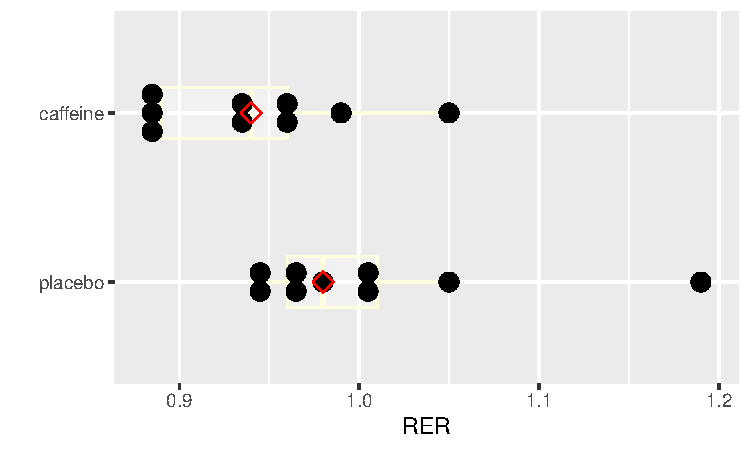
\includegraphics[width=\maxwidth]{htest-reraa-1} }

\caption[Two-sample parallel group RCT]{Data for two-sample RCT for effect of caffeine on respiratory exchange ratio. Diamonds depict medians.}\label{fig:htest-reraa}
\end{figure}
\end{Schunk}

\subsection{Frequentist $t$-Test}
To demonstrate difficulties in checking model assumptions with small $n$, consider the comprehensive approach by checking for linearity and parallelism (if equal variance assumption is used) of $z$-transformed empirical cumulative distributions.

\begin{Schunk}
\begin{Sinput}
Ecdf(~ log(rer), groups=tx, fun=qnorm, data=d,
     xlab='log(RER)', ylab='Inverse Normal ECDF')  # Fig. (*\ref{fig:htest-rerpass}*) 
\end{Sinput}
\begin{figure}[htbp]

\centerline{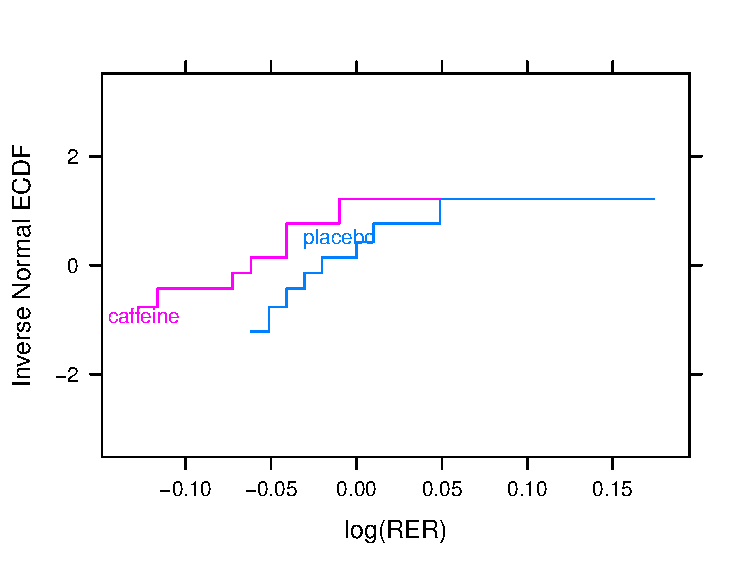
\includegraphics[width=\maxwidth]{htest-rerpass-1} }

\caption[Stratified ECDFs for checking $t$-test assumptions]{Stratified empirical cumulative distribution functions by treatment for checking all assumptions of the two-sample $t$-test.  ECDFs are inverse normal transformed.}\label{fig:htest-rerpass}
\end{figure}
\end{Schunk}

It is more accepted in practice to now use the form of the $t$-test
that does not assume equal variances in the two independent groups.
The unequal-variance $t$-test is used here.  Note that to compute a
decent approximation to the $P$-value requires the use of a ``trick''
d.f.\ when looking up against a $t$ distribution.
\begin{Schunk}
\begin{Sinput}
ttest <- t.test(log(rer) ~ tx, data=d)
# Note that for the CI t.test is using caffeine as the reference group
ttest
\end{Sinput}
\begin{Soutput}

	Welch Two Sample t-test

data:  log(rer) by tx
t = 2.0622, df = 15.337, p-value = 0.05655
alternative hypothesis: true difference in means is not equal to 0
95 percent confidence interval:
 -0.002027639  0.130381419
sample estimates:
 mean in group placebo mean in group caffeine 
           0.003115688           -0.061061202 
\end{Soutput}
\end{Schunk}
\bi
\item Interpretation
 \bi
 \item Subjects given caffeine have on average a log RER that is 0.064
   lower (0.95 CI: [-0.13, 0.002]) than individuals given placebo
 \item By anti-logging these 3 numbers we get the fold change scale:
   \bi
   \item Median\footnote{If the log ratio has a normal distribution,
       the log ratio has the same mean as the median and its
       median anti-logged value is the anti-log of the mean (=median)
       log difference.  The mean on the anti-logged scale is a more
       complex function that involves SD of log RER.} fold change is 0.94
   \item 0.95 CI for caffeine:placebo fold change: $[0.878, 1.002]$
   \ei
 \ei
\ei

\subsection{Bayesian $t$-Test}
The \R\ \Co{brms} package makes it easy to specify an unequal variance
model, because it allows one to specify a separate model for the log
of the standard deviation.  $\log(\sigma)$ can even depend on
continuous covariates!\footnote{Thanks to Nathan James of the
  Vanderbilt Department of Biostatistics for providing \R\ code for
  this section, and for providing the explanation for the output of
  the \co{prior\_summary} function.}  \co{brms} models standard
deviation parameters on the log scale.  As before, analysis is on the
log(RER) scale.
\begin{Schunk}
\begin{Sinput}
require(brms)
# set priors

# flat (non-informative) prior for intercept
pr0 <- set_prior("", class="Intercept")

# normal(0,3) prior for difference in log ratios
pr1 <- set_prior("normal(0,0.25)", class="b", coef="txcaffeine")

# normal(0,0.3912) for log SD ratio
pr2 <- set_prior("normal(0,0.3912)", class="b", coef="txcaffeine",
                 dpar="sigma")

# fit model for two groups assuming Y follows a t distribution so less 
# sensitive to outliers 
# Each group has different mean and SD but same df
# The prior for the log SD for the reference group is scale t with 3 d.f.
# Prior for nu is gamma(2, 0.1)
# The bf function is used to create a compound R model formula, here
# for the mean model and the log sigma model

f <- brm(bf(log(rer) ~ tx, sigma ~ tx), data=d, family=student,
            prior=c(pr0,pr1,pr2), seed=1202)
\end{Sinput}
\end{Schunk}

There are 5 parameters in this model (2 for the regression on student-$t$ mean, 2 for the regression on student-$t$ scale ($\sigma$), and 1 for student-$t$ d.f.\ $\nu$). The output from \co{prior\_summary()} shows all the parameters \emph{and} parameter classes that can be assigned. Lines 1 \& 3 in the output below are the `classes` of all non-intercept regression coefficients for the student-$t$ mean and student-$t$ scale, respectively. When there are multiple coefficients it is often convenient to specify a prior for all parameters in a class rather than for each individual parameter. For example, in a model with 10 covariates using \co{set\_prior("normal(0,1)", class="b")} would give each of the 10 corresponding coefficient parameters a standard normal prior. For our model the class priors are superseded by the individual parameter priors.
\begin{Schunk}
\begin{Sinput}
# Show priors in effect
prior_summary(f)
\end{Sinput}
\begin{Soutput}
                prior     class       coef group resp  dpar nlpar bound
1                             b                                        
2      normal(0,0.25)         b txcaffeine                             
3                             b                       sigma            
4    normal(0,0.3912)         b txcaffeine            sigma            
5                     Intercept                                        
6 student_t(3, 0, 10) Intercept                       sigma            
7       gamma(2, 0.1)        nu                                        
\end{Soutput}
\begin{Sinput}
# model summary
# Note: sigma is on log scale, use exp(sigma) to get to natural scale
# Intercept is mean for placebo
# sigma_Intercept is log(sd) for placebo
# txcaffeine is change in mean for caffeine compared to placebo
# sigma_txcaffeine is change in log(sd) for caffeine compared to placebo
f
\end{Sinput}
\begin{Soutput}
 Family: student 
  Links: mu = identity; sigma = log; nu = identity 
Formula: log(rer) ~ tx 
         sigma ~ tx
   Data: d (Number of observations: 18) 
Samples: 4 chains, each with iter = 2000; warmup = 1000; thin = 1;
         total post-warmup samples = 4000

Population-Level Effects: 
                 Estimate Est.Error l-95% CI u-95% CI Rhat Bulk_ESS Tail_ESS
Intercept           -0.00      0.02    -0.05     0.04 1.00     3747     2751
sigma_Intercept     -2.79      0.30    -3.43    -2.22 1.00     2642     2230
txcaffeine          -0.06      0.03    -0.12     0.01 1.00     4127     2533
sigma_txcaffeine    -0.05      0.30    -0.63     0.57 1.00     4114     2775

Family Specific Parameters: 
   Estimate Est.Error l-95% CI u-95% CI Rhat Bulk_ESS Tail_ESS
nu    18.17     14.05     2.28    53.10 1.00     2671     1753

Samples were drawn using sampling(NUTS). For each parameter, Eff.Sample 
is a crude measure of effective sample size, and Rhat is the potential 
scale reduction factor on split chains (at convergence, Rhat = 1).
\end{Soutput}
\begin{Sinput}
# plot kernel density est and trace plots for posterior parameters
plot(f)
\end{Sinput}


\centerline{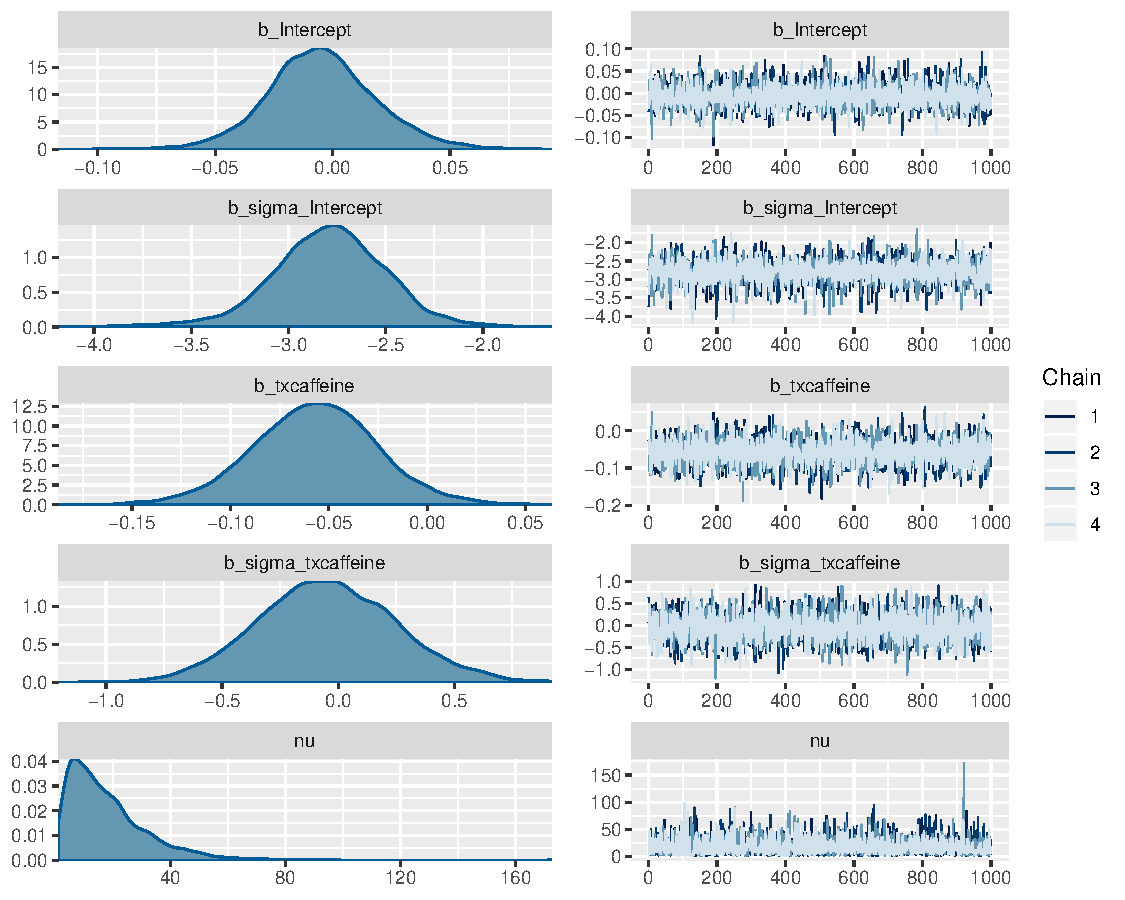
\includegraphics[width=\maxwidth]{htest-bayesfit2b-1} }

\end{Schunk}

\begin{Schunk}
\begin{Sinput}
# posterior predictive check
pp_check(f)
\end{Sinput}


\centerline{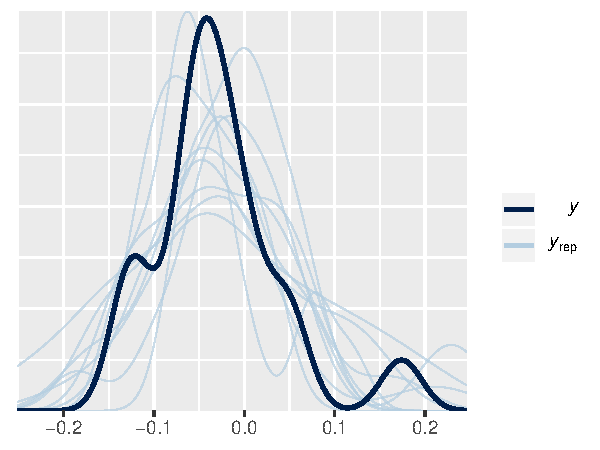
\includegraphics[width=\maxwidth]{htest-bayesfit2c-1} }

\end{Schunk}

\begin{Schunk}
\begin{Sinput}
# marginal effects 
plot(marginal_effects(f), points = TRUE)
\end{Sinput}


\centerline{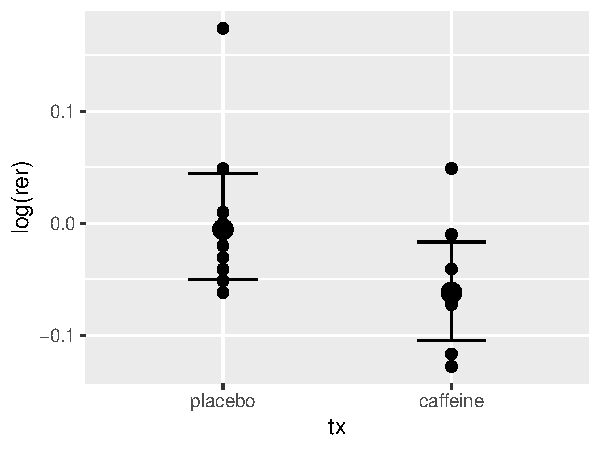
\includegraphics[width=\maxwidth]{htest-bayesfit2d-1} }

\end{Schunk}

\begin{Schunk}
\begin{Sinput}
# posterior parameter samples
p <- as.data.frame(f)
meanplacebo <- p[, 'b_Intercept']
delta       <- p[, 'b_txcaffeine']
sdplacebo   <- exp(p[, 'b_sigma_Intercept'])
sdratio     <- exp(p[, 'b_sigma_txcaffeine'])
nu          <- p[, 'nu']

# histogram of posterior distribution of difference in mean log RER
hist(delta, nclass=50, main='')

# Posterior density for caffeine:placebo fold change in RER
plot(density(exp(delta)), xlab='Fold Change in RER', main='')
abline(v=1, col=gray(0.85))

# Posterior density of SD ratio
plot(density(sdratio), main='', xlab='SD Ratio')
abline(v=1, col=gray(0.85))

# Posterior prob that difference in means < 0
# Recall that the P operator was defined previously
# (based on mean of logical or 0/1 values = proportion positive =
#  posterior probability to within simulation error
# This is the same as P(fold change < 1)
P(delta < 0)
\end{Sinput}
\begin{Soutput}
[1] 0.965
\end{Soutput}
\begin{Sinput}
P(exp(delta) < 1)
\end{Sinput}
\begin{Soutput}
[1] 0.965
\end{Soutput}
\begin{Sinput}
# Prob that caffeine results in a physiologically noticeable response
P(exp(delta) < 0.95)
\end{Sinput}
\begin{Soutput}
[1] 0.56825
\end{Soutput}
\begin{Sinput}
# Prob that caffeine and placebo have similar response
P(exp(delta) > 0.975 & exp(delta) < 1/0.975)
\end{Sinput}
\begin{Soutput}
[1] 0.141
\end{Soutput}
\begin{Sinput}
# Compute posterior probability of approximate normality
P(nu > 20)
\end{Sinput}
\begin{Soutput}
[1] 0.3535
\end{Soutput}


\centerline{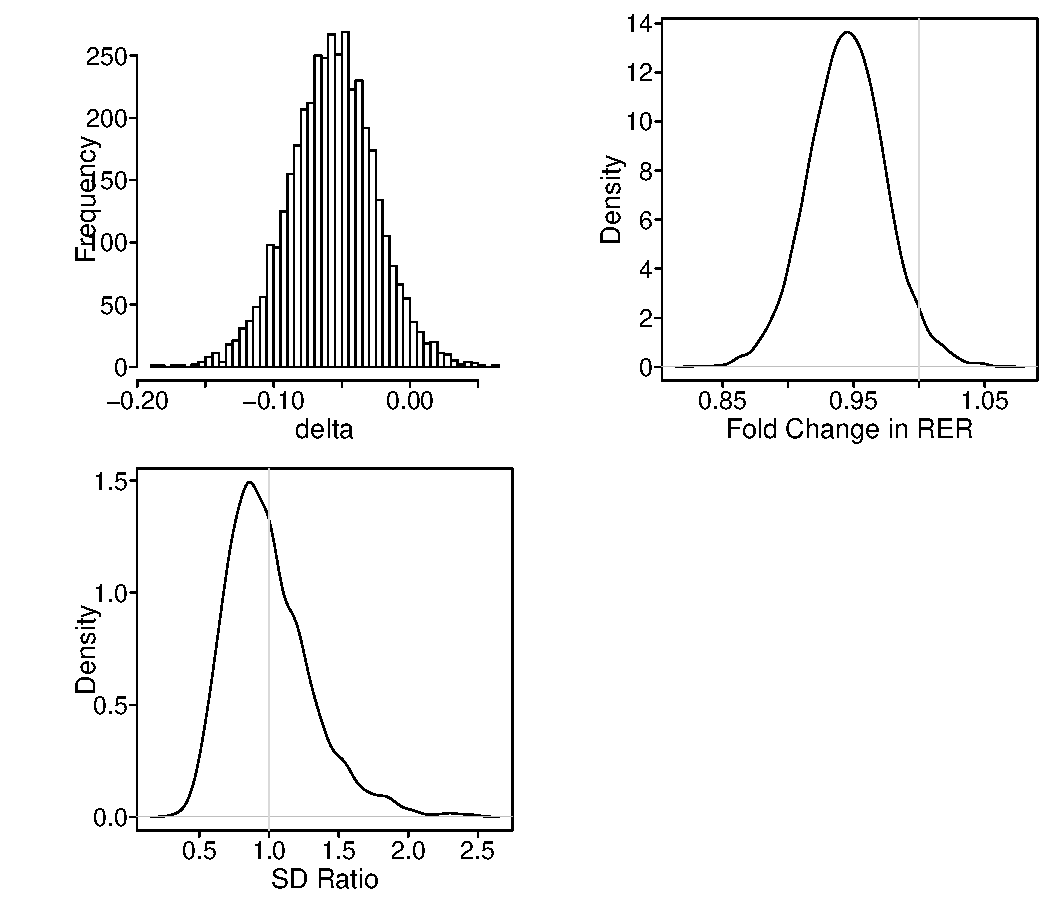
\includegraphics[width=\maxwidth]{htest-bayesfit2e-1} }

\end{Schunk}

Note that the
2-tailed $P$-value of 0.057 may tempt bright-line threshold advocates
to conclude nothing more than insufficient evidence to reject the
assumption that caffeine does not modify RER (or worse yet to just declare
an ``insigificant" result or even worse that caffeine does not modify
RER).  The Bayesian result shows that under a fairly skeptical prior
for log RER one would do well to play the odds in betting on caffeine
having an effect.

There is little evidence to support an assumption of normality of log
RER within a treatment group.

Now compare other results results with the frequentist analysis.  

\begin{Schunk}
\begin{Sinput}
means <- with(d, tapply(logrer, tx, mean))
sds   <- with(d, tapply(logrer, tx, sd))
a <- c(means[1],    pmode(meanplacebo), mean(meanplacebo), median(meanplacebo))
b <- c(sds[1],      pmode(sdplacebo),   mean(sdplacebo),   median(sdplacebo))
w <- c(diff(means), pmode(delta),     mean(delta),     median(delta))
z <- c(sds[2] / sds[1], pmode(sdratio), mean(sdratio), median(sdratio))
x <- rbind(a, b, w, z)
colnames(x) <- c('Sample', 'Posterior Mode', 'Posterior Mean',
                 'Posterior Median')
rownames(x) <- c('Placebo mean', 'Placebo SD', 'Caffeine - Placebo Mean',
                 'Caffeine / Placebo SD')
round(x, 2)
\end{Sinput}
\begin{Soutput}
                        Sample Posterior Mode Posterior Mean Posterior Median
Placebo mean              0.00          -0.01           0.00            -0.01
Placebo SD                0.07           0.06           0.06             0.06
Caffeine - Placebo Mean  -0.06          -0.06          -0.06            -0.06
Caffeine / Placebo SD     0.81           0.86           1.00             0.95
\end{Soutput}
\begin{Sinput}
# 0.95 credible interval for delta
quantile(delta, c(0.025, .975))
\end{Sinput}
\begin{Soutput}
        2.5%        97.5% 
-0.120428468  0.005351076 
\end{Soutput}
\begin{Sinput}
# 0.95 confidence interval for delta
rev(- ttest$conf.int)   # negate since t.test used different reference
\end{Sinput}
\begin{Soutput}
[1] -0.130381419  0.002027639
\end{Soutput}
\end{Schunk}

For an excellent tutorial on the use of \co{brms} for a two-sample $t$-test see \href{https://vuorre.netlify.com/post/2017/01/02/how-to-compare-two-groups-with-robust-bayesian-estimation-using-r-stan-and-brms}{bit.ly/brms-t} by Matti Vuorre


\section{The Problem with Hypothesis Tests and $P$-values Revisited}
\subsection{Hypothesis Testing}
\bi
\item Existence of ESP is a hypothesis
\item Assessing effects of drugs, procedures, devices involves
  estimation
\item Many studies powered to detect huge effect
\item If effect is not huge, no information from study
\ei

\subsection{$P$-Values} \ros{7.3}\altman{15-24}\abd{6.2}
\bi
\item Only provide evidence against a \emph{null} hypothesis,
  \textbf{never} evidence for something
\item Probability of a statistic \emph{more} impressive as yours \textbf{\Large
    if} $H_0$ true
\item Not a probability of an effect or difference (same problem with
  sensitivity and specificity)
\item \textbf{No} conclusion possible from large $P$-values
\item Cannot conclude clinical relevance from small $P$
\item Adjustment of $P$-values for multiple tests is controversial and
  there is insufficient consensus on how to choose an adjustment
  method
\item Declaring a result as ``significant'' or ``non-significant'' is completely arbitrary and has come to mean almost nothing
 \bi
  \item They rely on completely arbitrary $P$-value cutoffs such as 0.05
  \item American Statistical Association is on record recommending not using any cutoff or words like \emph{significant}: \href{https://amstat.tandfonline.com/doi/full/10.1080/00031305.2016.1154108}{bit.ly/asa-p} \href{https://www.tandfonline.com/doi/full/10.1080/00031305.2019.1583913}{bit.ly/asa-p2}
  \ei
\ei

\subsection{How Not to Present Results} \abd{6.2}
\bi
\item $P=0.02$ --- let's put this into clinical practice ignoring the
  drug's cost or clinical effectiveness
\item $P=0.4$ --- this drug does not kill people
\item $P=0.2$ but there is a trend in favor of our blockbuster drug
\item The observed difference was 6mmHg and we rejected $H_0$ so the
  true effect is 6mmHg.
\item The proportion of patients having adverse events was 0.01 and
  0.03; the study wasn't powered to detect adverse event differences
  so we present no statistical analysis
\item The reduction in blood pressure was 6mmHg with 0.95 C.L.\ of
  [1mmHg, 11mmHg]; the drug is just as likely to only reduce blood
  pressure by 1mmHg as it is by 6mmHg.
\item The serum pH for the 15 dogs was $7.3 \pm 0.1$ (mean $\pm$ SE instead of SD or IQR)
\ei

\subsection{How to Present Results} \altman{15-24}\abd{6.2}
\bi
\item Estimates should be accompanied by uncertainty intervals or posterior distributions
\item Confidence limits can be computed without regard to sample size
  or power
\item A computed value from a sample is only an estimate of the
  population value, whether or not you reject $H_0$
\item Best to think of an estimate from a study as a fuzz, not a point
\item To present variability of subjects, use SD or IQR, \textbf{not}
  SE (SE is the precision of the \emph{mean} of subjects)
\item If you must use $P$-values, provide the $P$-value to 3 significant digits and don't declare results as \emph{significant} or \emph{no significant difference}
\item See \href{https://discourse.datamethods.org/t/language-for-communicating-frequentist-results-about-treatment-effects}{http://bit.ly/datamethods-freq-results} for some guidelines for presenting frequentist results, and  \href{https://www.fharrell.com/post/bayes-freq-stmts}{fharrell.com/post/bayes-freq-stmts} for examples of Bayesian vs.\ frequentist summaries
\ei

\section{Study Design Considerations}\bmovie{7}\ddisc{7}
The majority of studies phrased as hypothesis testing experiments are
actually estimation studies, so it is usually preferred to based
sample size justifications on precision (margin of error).  Whether
using effect sizes in power calculations or margins of error in
precision calculations, the quantity of interest should be taken on
the original dependent variable scale or a transformation of it such
as odds or hazard.  

\subsection{Sizing a Pilot Study}
Frequently, pilot studies are used to obtain estimates of variability
that allow the sample sized to be calculated for a full study.  With a
continuous response variable, one can think of the adequacy of the
sample size in terms of the fold change or multiplicative margin of
error (MMOE) in the estimate $s$ of the population standard deviation $\sigma$.

When a sample of size $n$ is
drawn from a normal distribution, a $1 - \alpha$ two-sided confidence confidence
interval for the unknown population variance $\sigma^2$ is
given by
\begin{equation}
  \frac{n-1}{\chi^{2}_{1-\alpha/2,n-1}} s^{2} < \sigma^{2} <
  \frac{n-1}{\chi^{2}_{\alpha/2,n-1}} s^{2},
  \end{equation}
where $s^2$ is the sample variance and $\chi^{2}_{\alpha,n-1}$ is the
$\alpha$ critical value of the $\chi^2$ distribution with $n-1$
degrees of freedom.  The MMOE for estimating $\sigma$ is
\begin{equation}
  \sqrt{\max(\frac{\chi^{2}_{1-\alpha/2,n-1}}{n-1},
  \frac{n-1}{\chi^{2}_{\alpha/2,n-1}})}
\end{equation}
\begin{Schunk}
\begin{Sinput}
n    <- 10:300
low  <- sqrt((n - 1) / qchisq(.975, n - 1))
hi   <- sqrt((n - 1) / qchisq(.025, n - 1))
m    <- pmax(1 / low, hi)
ggplot(data.frame(n, m), aes(x=n, y=m)) + geom_line() +
  ylab('MMOE for s')
nmin <- min(n[m <= 1.2])
\end{Sinput}
\begin{figure}[htbp]

\centerline{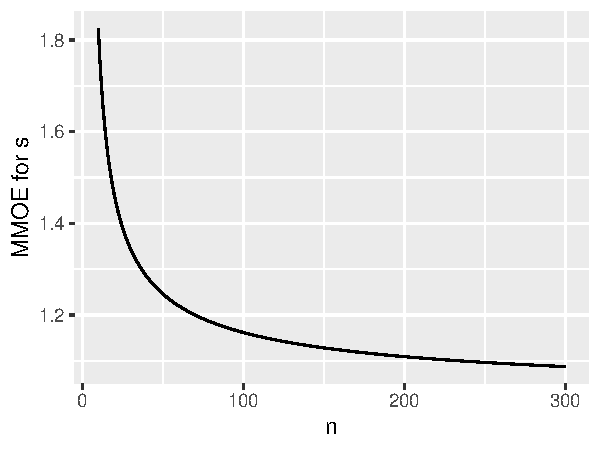
\includegraphics[width=\maxwidth]{htest-smmoe-1} }

\caption[Margin of error in estimating $\sigma$]{Multiplicative margin of error in estimating $\sigma$ as a function of sample size, with 0.95 confidence}\label{fig:htest-smmoe}
\end{figure}
\end{Schunk}
From the above calculations, to achieve a MMOE of no worse than 1.2
with 0.95 confidence when estimating $\sigma$ requires a sample size
of 70 subjects.  A pilot study with $n=20$ will achieve a
MMOE of 1.46 in estimating $\sigma$.

\subsection{Problems with Standardized Effect Sizes}
Many researchers use Cohen's standardized effect sizes in planning a
study. This has the advantage of not requiring pilot data. But such
effect sizes are not biologically meaningful and may hide important
issues~\cite{len01som}. Studies should be designed on the basis
of effects that are relevant to the investigator and human
subjects. If, for example, one plans a study to detect a one standard
deviation (SD) difference in the means and the SD is large, one can
easily miss a biologically important difference that happened to be
much less than one SD in magnitude. Note that the SD is a measure of
how subjects disagree with one another, not a measure of an effect
(e.g., the shift in the mean).  One way to see that standardized
effect sizes are problematic is to note that if one were to make the
measurements more noisy, the SD will increase and the purported
clinically important difference to detect will increase proportionately.

\subsection{Choice of Effect Size}
If a study is designed to detect a certain effect size with a given
power, the effect size should never be the observed effect from
another study, which may be estimated with error and be overly
optimistic. The effect size to use in planning should be the
clinically or biologically relevant effect one would regret
missing.  Usually the only information from prior studies that is
useful in sample size estimation are (in the case of a continuous
response variable with a symmetric distribution) estimates of the
standard deviation or the correlation between two measurements on the
same subject measured at two different times, or (in the case of a
binary or time to event outcome) event probabilities in control
subjects.  An excellent resource by Senn for understanding effect
sizes in power calculations may be found at \href{http://bit.ly/ssenn-effect}{bit.ly/ssenn-effect}.

\bi
\item Effect size for power/sample size calculation is \textbf{never} an observed effect in previous data
\item It is not the difference we believe is true
\item It is the difference you would not like to miss
\item Clinically relevant to patients or at least to physiology
\item Not \emph{greater than clinically relevant}
\ei

\subsection{Multiple Estimands and Hypotheses}\label{sec:htest-mult}
In many experiments there are more than one estimand (what is to be
estimated based on the question of interest) or hypothesis.  Some
frequentist statisticians and biomedical investigators believe that in such
situations the familywise error probability should be
controlled\footnote{As stated elsewhere, multiplicity adjustments are
  a byproduct of faults in frequentist inference and are completely arbitrary.}.
This probability is the probability of rejecting \emph{any} null
hypothesis given that \emph{all} null hypotheses are true.  One may
accomplish this by testing every hypothesis at the $\alpha^{*}$ level,
where the constant $\alpha^{*} < \alpha$ is chosen so that the overall
type one error is $\alpha$, or one may elect to
differentially ``spend $\alpha$'' by, for example, setting $\alpha=0.04$ for a
primary hypothesis and $\alpha=0.01$ for a less important secondary
analysis.  Another alternative is closed testing procedures whereby
later hypotheses can be tested at less stringent $\alpha$ levels as
long as all earlier hypotheses were rejected.  Unfortunately there is
no unique path to deriving multiplicity adjustments, and they have the
odd property of requiring one to be more stringent in assessing
evidence for one hypothesis just because one had other hypotheses.

An alternative, and what we believe to be more reasonable, view is by
Cook and Farewell~\cite{coo96mul} who stated that if a study has more
than one question and each question is to be answered on its own,
there is no need for a multiplicity adjustment.  This is especially
true if a strong priority ordering for hypotheses is stated in
advance.  For example, an investigator may specify three hypotheses about
efficacy of a treatment for the following
endpoints in a cardiovascular trial, sorted from most important to
least important: overall mortality, cardiovascular mortality,
and cardiovascular death or myocardial infarction.  As long as the
researcher always reports all of the results in context, in this
pre-specified order, each $P$-value can stand on its own.

Contrast this with an exploratory study in which the hypothesis is
essentially that there exists an endpoint for which the treatment is
effective.  One should expect to have to employ a conservative
multiplicity adjustment in that situation, e.g., Bonferroni's inequality.

Consider a frequentist study with four efficacy endpoints and corresponding $P$-values in the given pre-specified priority order: all-cause mortality ($P=0.09$), stroke ($P=0.01$), myocardial infarction ($P=0.06$), hospitalization ($P=0.11$)
\bi
\item  OK to quantify evidence against each of the 4 null hypotheses if all 4 reported in context, using the pre-specified order with separate interpretations
\item  Reasonable conclusion: With the current sample size, there is little evidence to reject the supposition that treatment does not lower mortality.  There is evidence against the supposition that treatment does not lower the rate of stroke. \ldots
\item  Contrast with a report that merely reports the stroke result, essentially saying ``there exists an endpoint for which treatment is effective''
\item Example Bayesian statement: Treatment probably (0.92) lowers mortality, probably (0.995) lowers the rate of stroke, probably (0.96) lowers MI, and probably (0.96) lowers hospitalization (posterior probabilities of a treatment benefit are in parentheses)\footnote{A Bayesian analysis would quickly add the (lower) probabilities that treatment lowers event rates by more than a trivial amount.  Bayesian methods can also compute the probability that any 2 of the efficacy targets were achieved, and the expected number of targets hit---in this case 0.92+0.995+0.96+0.96=3.8 of 4 targets hit.}.
\item Perhaps better: create a 5 or more level ordinal endpoint and use the worst event as the response variable
  \bi
  \item $Y=0, 1, 2, 3, 4$ corresponding to no event, hospitalization, MI, stroke, death
  \item Interpretation 1: treatment lowered the odds of an outcome or a worse outcome by a factor of 0.8
  \item Interpretation 2: chance of MI, stroke, or death with treatment estimated as 0.167 and for control as 0.2\\
    chances of stroke or death: 0.082, 0.1
  \item Bayesian probability of treatment benefit = $P(\textrm{OR} < 1) = 0.998$
  \ei
\item See Section \ref{sec:overview-ychoice} for how properties of ordinal scales relate to power
\ei

\subsection{Study Design Big Picture}\label{sec:htest-design-big}
\bi
\item Choose the right question or estimand
\item Think hard about subject/animal selection criteria
\item Decide whether you are doing a pilot study or a more definitive study
  \bi
  \item Pilot study is not used to nail down the effect of an intervention
  \item Is to show you can make the measurements, carry out the intervention, refine existing measurements, enroll enough subjects per month, etc.
  \item Power is not relevant
  \item May size the pilot study to be able to estimate something simple with precision (proportion, SD); adequate estimation of SD for continuous $Y$ is important for sample size calculation for the full study
  \ei
\item Make sure the design can answer that question were the sample size 1,000,000 subjects
\item Decide whether you are required to have a fixed sample size
 \bi 
 \item If budgeting is flexible, use fully sequential design and stop when evidence is adequate\footnote{Bayesian sequential designs require no penalty for infinitely many such data looks.  See \href{https://www.fharrell.com/post/bayes-seq}{fharrell.com/post/bayes-seq}.}
 \item For fixed budget/study duration be realistic about the effect size
 \ei 
\item If there is inadequate budget for detecting the minimal clinically important effect with high probability, be realistic about stating the study's likely yield
 \bi
 \item Best: compute the likely margin of error for the primary estimand
 \item Next best: compute the power that will be achieved with the limited sample size
 \ei
\item Choose a response variable $Y$ that answers the question and has the greatest frequentist or Bayesian power (section \ref{sec:overview-ychoice}))
  \bi
  \item Example: primary interest is patient's inability to function physically on a 0-100 scale (100=bedridden)
  \item Some patients will be too sick to have their function assessed and some will die
\setcounter{footnote}{0}
  \item Define $Y$=0-100 overridden with 101 for too sick or 102 for death\footnote{Ordinal analysis will not be affected by placing the clinical events at 1001 and 1002 or any other levels that are higher than the highest functional disability level.}
  \item Analyze with the proportional odds model
  \item Interpretation:
   \bi
   \item Primary endpoint is degree of functional disability, penalized by death or being physically unable to be assessed
   \item Proportional odds model provides an overall odds ratio for treatments B:A (ratio of odds that $Y \geq j$ for any $j$)
   \item Model can also be used to estimate the median disability, where sickness or death will shift the median to the right a little
   \item May also be summarized by estimating for each treatment the probability that a patient has level 50 functional disability or worse where ``or worse'' means 51-100, too sick, or dead, after estimating the overall odds ratio for treatment
   \ei
  \ei
\item Use multiple measurements over time to increase power/precision and to allow more questions to be answered
\item Greatest power comes from having a continuous $Y$ or ordinal $Y$ with many well-populated levels, where $Y$ is also measured at baseline and is adjusted for as a covariate in ANCOVA, allowing for a smooth nonlinear effect (without assuming the slope is 1.0 as is assumed by change-from-baseline analysis)
\item Never use change from baseline as the response variable except in a non-randomized pre-post design (the weakest of all designs)
\item If treatment is short-term and wears off, fully using each subject as her own control in a randomized crossover study may be ideal
\item For a parallel-group randomized study, accurately collect key baseline variables that explain outcome heterogeneity
\item For an observational study, accurately capture a host of baseline variables that are likely to result in adequate confounder adjustment
 \bi
 \item don't merely rationalize that variables available in an existing dataset are adequate
 \ei
\item Use a research data management tool such as REDCap that allows for extensive data quality checking
\item Don't forget the many subject selection, ethical, and good clinical practice issues
\item Recommended reading: Hulley~\etal~\emph{Designing Clinical Research}~\cite{hul13des}
\ei 

\section{One-Sample $t$-Test Revisited}

\subsection{Study Description}

\bi
\item Compare the effects of two soporific drugs (optical isomers of hyoscyamine hydrobromide)
\item Crossover study
\item Each subject receives placebo run-in, then Drug 1, then Drug 2
\item Investigator may not have randomized order of treatments
\item Dependent variable: Number of hours of increased sleep when
  compared to a placebo run-in period (raw data not shown)
\item Drug 1 given to $n$ subjects, Drug 2 given to same $n$ subjects
\item Study question: Is Drug 1 or Drug 2 more effective at increasing sleep?
  \bi
  \item $H_0: \mu_d = 0 \hspace{.2cm} \textrm{where} \hspace{.2cm} \mu_d = \mu_1 - \mu_2$
  \item $H_1: \mu_d \neq 0$
  \ei
\ei


\subsection{Power and Sample Size}

\bi
\item Pilot study or previous published research shows the standard deviation of the difference ($\sigma_d$) is $1.2$ hours
\item Determine the number of subjects needed for several value of effect size $\Delta$ ($\Delta = |\mu_1 - \mu_2|$)with 0.9 power, $\alpha = 0.05$
\ei

 \begin{center}
 \begin{tabular}{lrrrr}\hline\hline
$\Delta$ &$ 0.5$&$ 1$&$1.5$&$2$\\
$n$ &$62$&$16$&$8$&$5$\\
\hline
\end{tabular}
\end{center}

\bi
\item If Drug 1 (or 2) increases sleep by 1.5 hours more than Drug 2 (or 1), by enrolling 8 subjects we will have 0.9 power to detect an association.
\item More powerful than the two sample test (need 10 subjects in each group for $\Delta = 3.0$ hours)
\ei
\subsection{Collected Data}
Here are the data for the 10 subjects.  This is the \R\ built-in dataset \co{sleep}.
 \begin{center}
 \begin{tabular}{lrrr}\hline\hline
Subject & Drug 1 & Drug 2 & {\color{red}Diff (2-1)}
\\ \hline
1 & $ 0.7$&$ 1.9$&$\color{red}1.2$\\
2 &$-1.6$&$ 0.8$&$\color{red}2.4$\\
3 &$-0.2$&$ 1.1$&$\color{red}1.3$\\
4 &$-1.2$&$ 0.1$&$\color{red}1.3$\\
5 &$-0.1$&$-0.1$&$\color{red}0.0$\\
6 &$ 3.4$&$ 4.4$&$\color{red}1.0$\\
7 &$ 3.7$&$ 5.5$&$\color{red}1.8$\\
8 &$ 0.8$&$ 1.6$&$\color{red}0.8$\\
9 &$ 0.0$&$ 4.6$&$\color{red}4.6$\\
10 &$ 2.0$&$ 3.4$&$\color{red}1.4$\\ \\
Mean & $ 0.75$&$ 2.33$&$\color{red}1.58$\\
SD & $ 1.79$&$ 2.0$&$\color{red}1.2$\\
\hline
\end{tabular}\alabel{sleeppaired}
\end{center}

\begin{Schunk}
\begin{Sinput}
drug1 <- c(.7, -1.6, -.2, -1.2, -.1, 3.4, 3.7, .8, 0, 2)
drug2 <- c(1.9, .8, 1.1, .1, -.1, 4.4, 5.5, 1.6, 4.6, 3.4)
d <- data.frame(Drug=c(rep('Drug 1', 10), rep('Drug 2', 10),
                  rep('Difference', 10)),
                extra=c(drug1, drug2, drug2 - drug1))
w <- data.frame(drug1, drug2, diff=drug2 - drug1)

ggplot(d, aes(x=Drug, y=extra)) +   # Fig. (*\ref{fig:htest-tplot}*)
  geom_boxplot(col='lightyellow1', alpha=.3, width=.5) + 
  geom_dotplot(binaxis='y', stackdir='center', position='dodge') +
  stat_summary(fun.y=mean, geom="point", col='red', shape=18, size=5) +
  geom_segment(data=w, aes(x='Drug 1', xend='Drug 2', y=drug1, yend=drug2),
               col=gray(.8)) +
  geom_segment(data=w, aes(x='Drug 1', xend='Difference', y=drug1, yend=drug2 - drug1),
               col=gray(.8)) +
  xlab('') + ylab('Extra Hours of Sleep') + coord_flip() 
\end{Sinput}
\begin{figure}[htbp]

\centerline{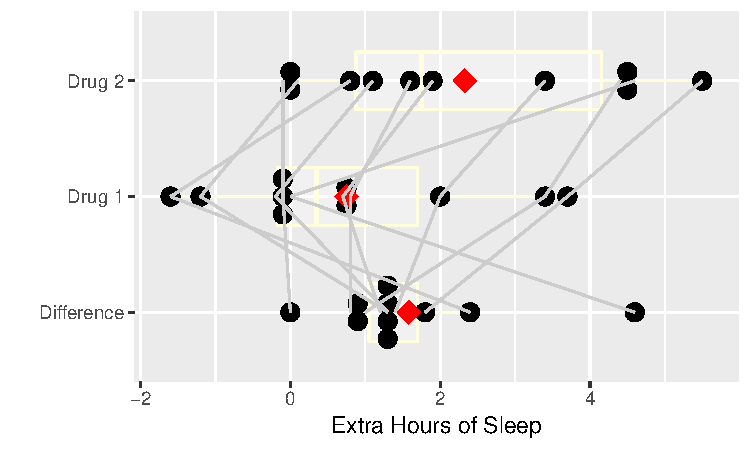
\includegraphics[width=\maxwidth]{htest-tplot-1} }

\caption[Data and box plots for paired data]{Raw data and box plots for paired data and their paired differences, with lines connecting points from the same subject.  Diamonds depict means.}\label{fig:htest-tplot}
\end{figure}
\end{Schunk}

\subsection{Statistical Test}
\begin{Schunk}
\begin{Sinput}
with(d, t.test(drug1, drug2, paired=TRUE))
\end{Sinput}
\begin{Soutput}

	Paired t-test

data:  drug1 and drug2
t = -4.0621, df = 9, p-value = 0.002833
alternative hypothesis: true difference in means is not equal to 0
95 percent confidence interval:
 -2.4598858 -0.7001142
sample estimates:
mean of the differences 
                  -1.58 
\end{Soutput}
\end{Schunk}
\bi
\item Interpretation
 \bi
 \item A person who takes Drug 2 sleeps on average 1.58 hours longer (0.95 CI: [0.70, 2.46]) than a person who takes Drug 1
 \ei
%\item Note: Same point estimate (1.58 hours), but more precise estimate (tighter CI) than the 2-sample $t$-test
\ei

\clearpage
\section{Comprehensive Example: Crossover Design and Analysis}
\bi
 \item In the previous example, it was not clear if the order of placebo, Drug 1, and Drug 2 was the same for every patient
 \item In a crossover design, each patient receives both drugs
   \bi
     \item Can serve as own control
     \item Effectively adjusts for all baseline variables without measuring them\footnote{If there is no interaction between covariate and treatment order}
     \item Order is randomized
   \ei
 \item Carryover effects
   \bi
      \item Def: An effects that carries over from one experimental condition to another
      \item Need a washout period between drugs to remove carryover effects
      \item Time to remove carryover effects should be based on biology, not statistics
      \item Statistical tests for carryover effects are often not
        precise enough to make definitive conclusions (see example) 
      \item The test for carryover is correlated with the overall
        test of efficacy
      \item Pre-testing for carryover then deciding whether to only
        use phase 1 data results in a huge inflation of type I error
        in the test for efficacy
   \ei
\ei

\subsection{Study Description}

\bi
\item Compare the effects of two soporific drugs.
\item Each subject either (1) starts with Drug 1 and crosses over to Drug 2 or (2) starts with Drug 2 and crosses over to Drug 1
  \bi
    \item No placebo run-in in this example
    \item Order randomly assigned
    \item Suitable period of time ($\sim 5$ half-lives) between drug
      crossovers to washout effects of previous drug 
  \ei
\item Dependent variable: Number of hours of sleep on each drug
\item Drug 1 given to $n$ subjects, Drug 2 given to same $n$ subjects
\item Study question: Is Drug 1 or Drug 2 more effective at increasing sleep?
  \bi
  \item $H_0: \mu_d = 0 \hspace{.2cm} \textrm{where} \hspace{.2cm} \mu_d = \mu_1 - \mu_2$
  \item $H_1: \mu_d \neq 0$
  \ei
\ei


\subsection{Power and Sample Size}

\bi
\item Pilot study or previous published research shows the standard deviation of the difference ($\sigma_d$) is $1.2$ hours
\item Determine the number of subjects needed for several value of effect size $\Delta$ ($\Delta = |\mu_1 - \mu_2|$)with 0.9 power, $\alpha = 0.05$
\item Assume no carryover effects
\ei

 \begin{center}
 \begin{tabular}{lrrrr}\hline\hline
$\Delta$ &$ 0.5$&$ 1$&$1.5$&$2$\\
$n$ &$62$&$16$&$8$&$5$\\
\hline
\end{tabular}
\end{center}

\bi
\item If Drug 1 (or 2) increases sleep by 1.5 hours more than Drug 2 (or 1), by enrolling 8 subjects we will have 0.9 power to detect an association.
\item Same power calculation as paired $t$-test
\ei

\subsection{Collected Data}
 \begin{center}
 \begin{tabular}{lrrr}\hline\hline
Subject & Drug 1 & Drug 2 & {\color{red}Diff (2-1)}
\\ \hline
1  &$8.7$ &$ 9.9$&$\color{red}1.2$\\
2  &$6.4$ &$ 8.8$&$\color{red}2.4$\\
3  &$7.8$ &$ 9.1$&$\color{red}1.3$\\
4  &$6.8$ &$ 8.1$&$\color{red}1.3$\\
5  &$7.9$ &$ 7.9$&$\color{red}0.0$\\
6  &$11.4$&$ 12.4$&$\color{red}1.0$\\
7  &$11.7$&$ 13.5$&$\color{red}1.8$\\
8  &$8.8$ &$ 9.6$&$\color{red}0.8$\\
9  &$8.0$ &$ 12.6$&$\color{red}4.6$\\
10 &$10.0$&$ 11.4$&$\color{red}1.4$\\ \\
Mean&$8.75$&$ 10.33$&$\color{red}1.58$\\
SD  &$1.79$&$ 2.0$  &$\color{red}1.2$\\
\hline
\end{tabular}
\end{center}

\subsection{Statistical Tests}
\begin{Schunk}
\begin{Sinput}
drug1 <- c(87, 64, 78, 68, 79, 114, 117, 88, 80, 100)/10
drug2 <- c(99, 88, 91, 81, 79, 124, 135, 96, 126, 114)/10
t.test(drug1, drug2, paired=TRUE)
\end{Sinput}
\begin{Soutput}

	Paired t-test

data:  drug1 and drug2
t = -4.0621, df = 9, p-value = 0.002833
alternative hypothesis: true difference in means is not equal to 0
95 percent confidence interval:
 -2.4598858 -0.7001142
sample estimates:
mean of the differences 
                  -1.58 
\end{Soutput}
\end{Schunk}
\bi
\item Interpretation
 \bi
 \item A person who takes Drug 2 sleeps on average 1.58 hours longer (0.95 CI: [0.70, 2.50]) than a person who takes Drug 1
 \ei
\ei

\subsection{Carryover Effects}

\bi
   \item Is there any evidence for a carryover effect?
   \item Assume that the first 5 subjects received Drug 1 first and the second 5 subjects received drug 2 first
   \item If we assume there are no carryover effects, then the mean difference in sleep for subjects receiving drug 1 first should be \textit{the same} as the mean difference for subjects receiving drug 2 first
   \item Assessing carryover effect distorts the efficacy
     analysis inference
   \item Null hypothesis is that there are no carryover effects
   \item Can rearrange the difference data to clarify the structure
\ei

 \begin{center}
 \begin{tabular}{lrr}\hline\hline
Subject & Drug 1 First & Drug 2 First
\\ \hline
1 & $\color{red}1.2$ & \\
2 & $\color{red}2.4$ & \\
3 & $\color{red}1.3$ & \\
4 & $\color{red}1.3$ & \\
5 & $\color{red}0.0$ & \\
6 & & $\color{red}1.0$\\
7 & & $\color{red}1.8$\\
8 & & $\color{red}0.8$\\
9 & & $\color{red}4.6$\\
10 & & $\color{red}1.4$\\ \\
Mean & 1.24 & 1.92 \\
SD & 0.85 & 1.55 \\
\hline
\end{tabular}
\end{center}

For this design we might expect the variance of the differences to be
the same for both orders, so we use the equal-variance $t$-test.
\begin{Schunk}
\begin{Sinput}
# Unpaired t-test
t.test((drug2 - drug1)[1:5], (drug2 - drug1)[6:10], var.equal=TRUE)
\end{Sinput}
\begin{Soutput}

	Two Sample t-test

data:  (drug2 - drug1)[1:5] and (drug2 - drug1)[6:10]
t = -0.86152, df = 8, p-value = 0.414
alternative hypothesis: true difference in means is not equal to 0
95 percent confidence interval:
 -2.500137  1.140137
sample estimates:
mean of x mean of y 
     1.24      1.92 
\end{Soutput}
\end{Schunk}
\bi
\item Interpretation
 \bi
 \item Large $P$-value has no interpretation
 \item With 0.95 confidence, the carryover effect is between [-2.5 and 1.1] hours, which is not scientifically convincing either way
 \item In general, be very cautious when the null hypothesis is something you want to fail to reject in order to validate your analysis method
   \bi
     \item Tests of normality are sometimes used to validate using a parametric over a non-parametric test
     \item There are also statistical tests for equal variance
     \item Both tests may be unreliable and will distort the final
       inference that is conditional on preassessments being correct
   \ei
 \ei
 \item As \href{https://www.amazon.com/Cross-over-Trials-Clinical-Research-Stephen/dp/0471496537}{Stephen Senn} has warned, be wary of doing anything
   about empirically quantified carryover effects, as the carryover
   effect estimate has a correlation of $\frac{1}{2}$ with the overall
   treatment effect estimate, causing the carryover test to ruin the
   operating characteristics of the treatment test
\ei

\subsection{Bayesian Analysis}

\bi
\item Reasonable to put prior knowledge on parameters, especially carryover event
\item Reasonable to restrict carryover effect to be less than the treatment effect
\item For related discussions and references for Bayesian crossover analysis see\\ \href{http://bit.ly/datamethods-bbr7}{bit.ly/datamethods-bbr7}
\ei
